%  compress using: gs -sDEVICE=pdfwrite -dCompatibilityLevel=1.4 -dNOPAUSE -dQUIET -dBATCH      -sOutputFile=IROS2017mappingComp.pdf IROS2017mapping.pdf

%\documentclass[conference]{IEEEtran}
\documentclass[letterpaper, 10 pt, conference]{ieeeconf}
\IEEEoverridecommandlockouts% This command is only needed if 
                                                          % you want to use the \thanks command
%\overrideIEEEmargins                                      % Needed to meet printer requirements.
\usepackage{times}


\makeatletter 
\let\NAT@parse\undefined
\makeatother

% numbers option provides compact numerical references in the text. 
%\usepackage[numbers]{natbib}
\usepackage{multicol}
\usepackage[bookmarks=true]{hyperref}

\usepackage{bbm}
\usepackage{calc}
\usepackage{url}
\usepackage{hyperref}
\hypersetup{
  colorlinks =false,
  urlcolor = black,
  linkcolor = black
}
\usepackage{graphicx}
\usepackage[cmex10]{amsmath}
\usepackage{bm}
\usepackage{amssymb}
\usepackage{rotating}
\usepackage{balance}
\usepackage{chngcntr}
\counterwithin{paragraph}{subsection} % makes paragraph depend on subsection


%\usepackage{xfrac}
\usepackage{nicefrac}
\usepackage{cite}
\usepackage[caption=false,font=footnotesize]{subfig}
\usepackage[usenames, dvipsnames]{color}
\usepackage{colortbl}
\usepackage{overpic}
\graphicspath{{./pictures/pdf/},{./pictures/ps/},{./pictures/png/},{./pictures/jpg/}}
\usepackage{breqn} %for breaking equations automatically
\usepackage[ruled]{algorithm}
\usepackage{algpseudocode}
%\usepackage{algorithmic}
\usepackage{multirow}
%\usepackage{todonotes}
\usepackage{authblk}

\newcommand{\todo}[1]{\vspace{5 mm}\par \noindent \framebox{\begin{minipage}[c]{0.98 \columnwidth} \ttfamily\flushleft \textcolor{red}{#1}\end{minipage}}\vspace{5 mm}\par}
% uncomment this to hide all red todos
%\renewcommand{\todo}{}

%% ABBREVIATIONS
\newcommand{\qstart}{q_{\text{start}}}

%% MACROS

\providecommand{\pmax}{ \overline{p} }   %p_{\text{max}}
\providecommand{\pmin}{ \underline{p} }   %p_{\text{min}}
\providecommand{\abs}[1]{\left\lvert#1\right\rvert}
\providecommand{\norm}[1]{\left\lVert#1\right\rVert}
\providecommand{\normn}[2]{\left\lVert#1\right\rVert_#2}
\providecommand{\dualnorm}[1]{\norm{#1}_\ast}
\providecommand{\dualnormn}[2]{\norm{#1}_{#2\ast}}
\providecommand{\set}[1]{\lbrace\,#1\,\rbrace}
\providecommand{\cset}[2]{\lbrace\,{#1}\nobreak\mid\nobreak{#2}\,\rbrace}
\providecommand{\lscal}{<}
\providecommand{\gscal}{>}
\providecommand{\lvect}{\prec}
\providecommand{\gvect}{\succ}
\providecommand{\leqscal}{\leq}
\providecommand{\geqscal}{\geq}
\providecommand{\leqvect}{\preceq}
\providecommand{\geqvect}{\succeq}
\providecommand{\onevect}{\mathbf{1}}
\providecommand{\zerovect}{\mathbf{0}}
\providecommand{\field}[1]{\mathbb{#1}}
\providecommand{\C}{\field{C}}
\providecommand{\R}{\field{R}}
\newcommand{\Cspace}{\mathcal{Q}}
\newcommand{\Uspace}{\mathcal{U}}
\providecommand{\Fspace}{\Cspace_\text{free}}
\providecommand{\Hcal}{$\mathcal{H}$}
\providecommand{\Vcal}{$\mathcal{V}$}
\DeclareMathOperator{\conv}{conv}
\DeclareMathOperator{\cone}{cone}
\DeclareMathOperator{\homog}{homog}
\DeclareMathOperator{\domain}{dom}
\DeclareMathOperator{\range}{range}
\DeclareMathOperator{\sign}{sgn}
\providecommand{\polar}{\triangle}
\providecommand{\ainner}{\underline{a}}
\providecommand{\aouter}{\overline{a}}
\providecommand{\binner}{\underline{b}}
\providecommand{\bouter}{\overline{b}}
\newcommand{\D}{\nobreakdash-\textsc{d}}
%\newcommand{\Fspace}{\mathcal{F}}
\providecommand{\Fspace}{\Cspace_\text{free}}
\providecommand{\free}{\text{\{}\mathsf{free}\text{\}}}
\providecommand{\iff}{\Leftrightarrow}
\providecommand{\subinner}[1]{#1_{\text{inner}}}
\providecommand{\subouter}[1]{#1_{\text{outer}}}
\providecommand{\Ppoly}{\mathcal{X}}
\providecommand{\Pproj}{\mathcal{Y}}
\providecommand{\Pinner}{\subinner{\Pproj}}
\providecommand{\Pouter}{\subouter{\Pproj}}
\DeclareMathOperator{\argmax}{arg\,max}
\providecommand{\Aineq}{B}
\providecommand{\Aeq}{A}
\providecommand{\bineq}{u}
\providecommand{\beq}{t}
\DeclareMathOperator{\area}{area}
\newcommand{\contact}[1]{\Cspace_{#1}}
\newcommand{\feasible}[1]{\Fspace_{#1}}
\newcommand{\dd}{\; \mathrm{d}}
\newcommand{\figwid}{0.22\columnwidth}
\newcommand{\TRUE}{\textbf{true}}
\newcommand{\FALSE}{\textbf{false}}
\DeclareMathOperator{\atan2}{atan2}
\allowdisplaybreaks

\newtheorem{theorem}{Theorem}
\newtheorem{definition}[theorem]{Definition}
\newtheorem{lemma}[theorem]{Lemma}


\pdfinfo{
   /Author (Arun Mahadev, Dominik Krupke, S\'{a}ndor P.~Fekete, and Aaron T. Becker)
   /Title  (Mapping, Foraging, and Coverage with a Particle Swarm Controlled by Uniform Inputs)
   /CreationDate (D:20160129120000)
   /Subject (Simple Robots)
   /Keywords (Robots;Uniform Control Inputs)
}


% paper title
\title{\LARGE \bf Mapping, Foraging, and Coverage\\ with a Particle Swarm Controlled by Uniform Inputs}

% You will get a Paper-ID when submitting a pdf file to the conference system
\author{Arun Mahadev, Dominik Krupke, S\'{a}ndor P.~Fekete, and Aaron T. Becker% <-this % stops a space
\thanks{*This work was supported by the National Science Foundation under Grant No.\ \href{http://nsf.gov/awardsearch/showAward?AWD_ID=1553063}{ [IIS-1553063]} and \href{http://nsf.gov/awardsearch/showAward?AWD_ID=1619278}{[IIS-1619278]}.}% <-this % stops a space
\thanks{A.~Mahadev and A.~Becker are with the Department of Electrical and Computer Engineering,  University of Houston, Houston, TX 77204-4005 USA 
      \protect\url{ aviswanathanmahadev@uh.edu,atbecker@uh.edu }}
\thanks{S.~Fekete and D.~Krupke are with the Dept.~of Computer Science, TU Braunschweig,  M\"uhlenpfordtstr.~23, 38106 Braunschweig, Germany,
      \protect\url{s.fekete@tu-bs.de,d.krupke@tu-bs.de  }
} %\end thanks%
}
\begin{document}



\maketitle
\thispagestyle{empty}
\pagestyle{empty}


\begin{abstract}
We propose a novel approach to mapping tissue and vascular systems without the use of contrast agents,
based on moving and measuring magnetic particles.
To this end, we consider a swarm of particles in a 1D or 2D grid that can be tracked and controlled by an external agent. 
Control inputs are applied uniformly so that each particle experiences the same applied forces. 
We present algorithms for three tasks: (1) {\em Mapping}, i.e., building a representation of the free and obstacle regions of the workspace;
(2) {\em Foraging}, i.e., ensuring that at least one particle reaches each of a set of desired locations; 
and (3) {\em Coverage}, i.e., ensuring that every free region on the map is visited by at least one particle.
These tasks relate to a large body of previous work from robot navigation, both from theory and practice, 
which is based on individual control.

We provide a spectrum of theoretical and practical new insights 
that have particular relevance for fast MRI scans with magnetically controlled contrast media.
In particular, we develop a fundamentally new approach 
for searching for an object (a {\em membrane} in the context of tissue) at an unknown distance $D$, where the search is 
subject to two different and independent cost parameters
for {\em moving} and for {\em measuring}. We show that regardless of the relative cost of these two operations,
there is a simple $O(\log D/\log\log D)$-competitive strategy, which is best possible.
We extend this to to other settings. In addition, we provide alternative, practically useful strategies for higher-dimensional
settings, as well as experimental results.
These algorithms extend to any number of particles, and show that additional
particles tend to reduce the mean and the standard deviation of the time required for each task.  %ADD MORE ABOUT EXPERIMENTS?
%In the limit, as the
%particle count increases, the time reduces to four moves for mapping and zero
%moves for foraging and coverage. 

%Algorithms are tested in simulation, and validated with hardware experiments using magnetically steered paramagnetic particles.
%These methods may have particular relevance for fast MRI scans with magnetically controlled contrast media.

% KEYWORDS:   uniform control, under-actuation, particle swarm
\end{abstract}

\IEEEpeerreviewmaketitle
%%%%%%%%%%%%%%%
\section{Introduction}\label{sec:Intro}
In MR imaging, some tissues have poor \emph{contrast}, which means that the boundaries between tissue types cannot be determined.
 To discover tissue boundaries, particulate solutions of a contrast agent are used to illuminate regions of interest~\cite{na2009inorganic}. 
 Drawbacks include that the contrast agent diffuses quickly and must be injected repeatedly during long scans. 
 Additionally, many contrast agents such as gadolinium chelates are toxic, and prolonged exposure causes medical complications \cite{caravan1999gadolinium}. 
This paper explores using steerable magnetic microparticles to map a region. 
These particles can be steered by the global magnetic gradient of an MRI and visualised by the MRI \cite{Vartholomeos2012}, even when the tissues they move through  have poor contrast.
As a current example for micro- and nano-particles that can be manufactured in large numbers, see~\cite{Chowdhury2015,martel2014computer,kim2015imparting,Donald2013,Ghosh2009,Ou2013,qiu2015magnetic}.

\begin{figure}
\begin{center}
	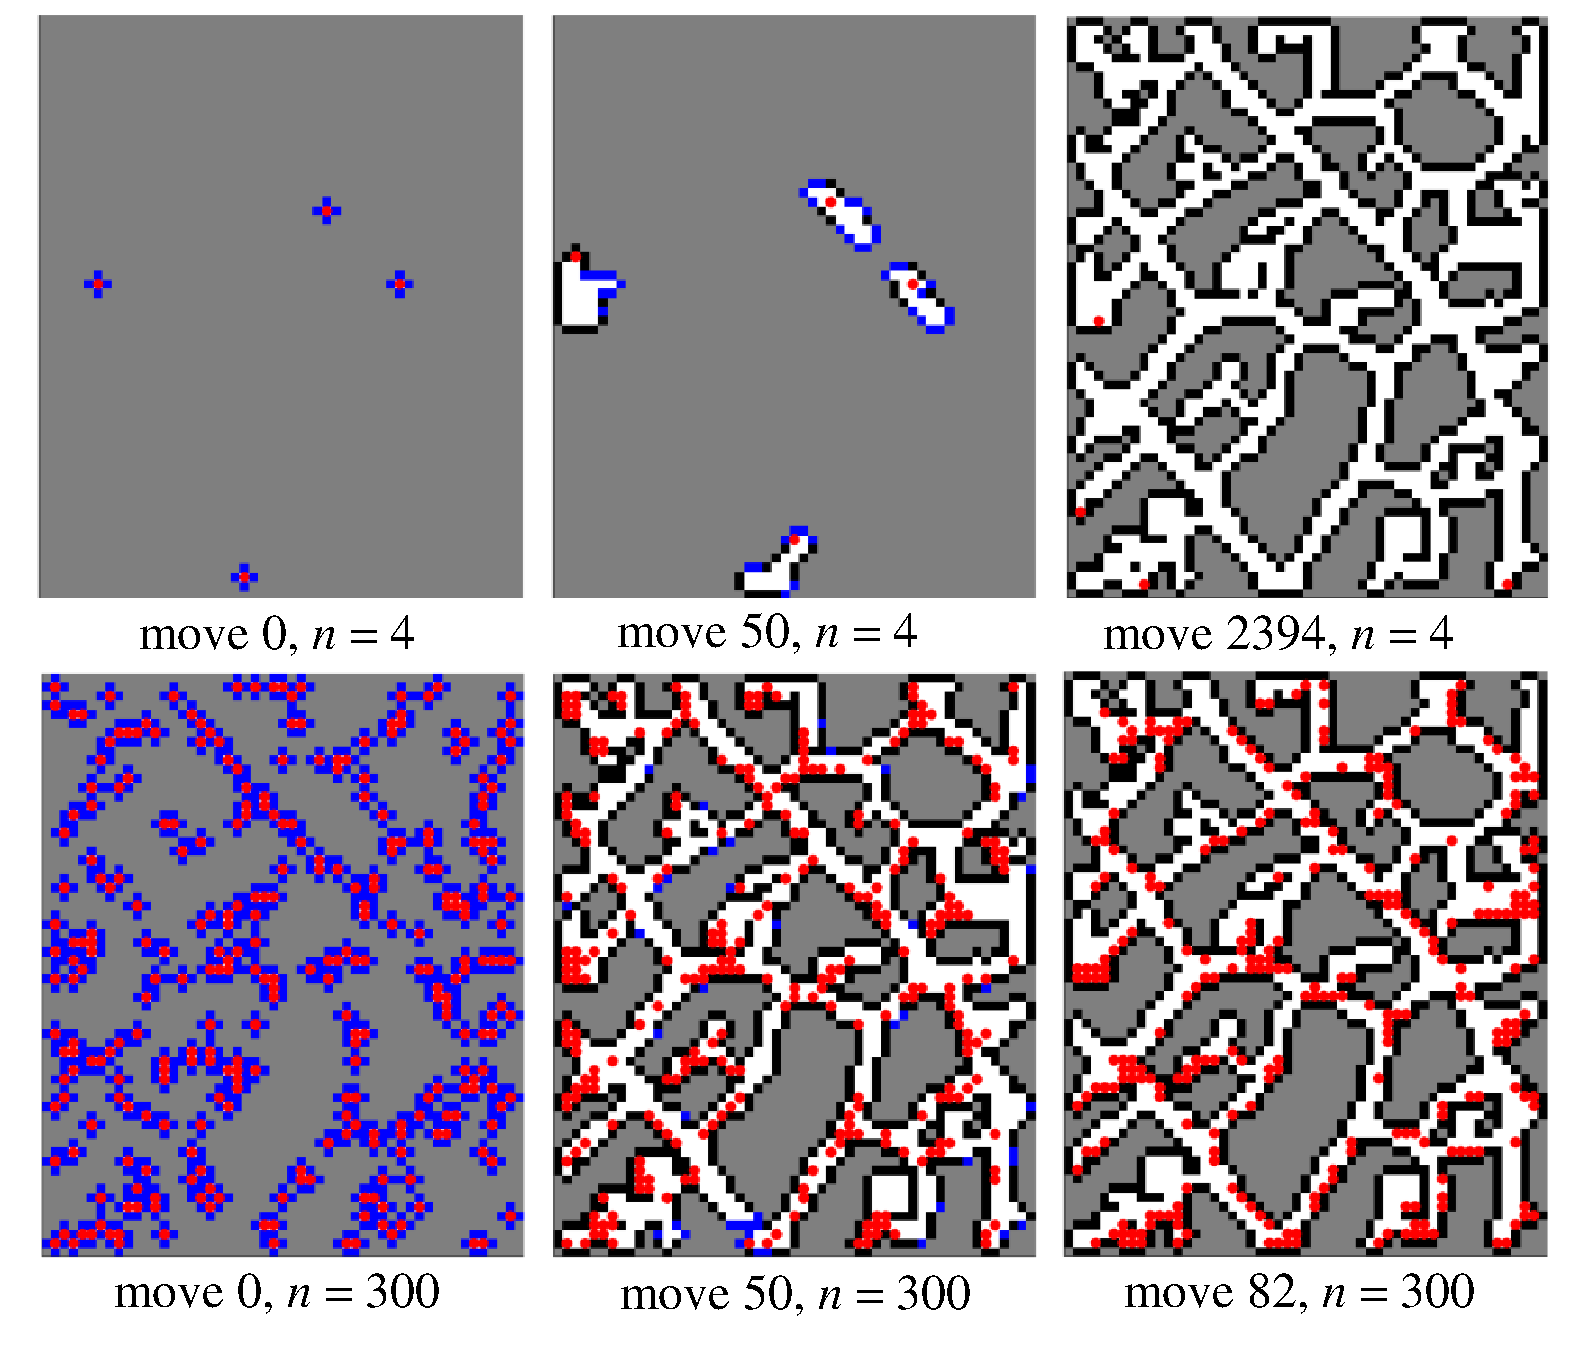
\includegraphics[width=1.0\columnwidth]{Coverage2DwithUnformControl1}
\end{center}
\caption{\label{fig:Coverage2DwithUnformControl}
Mapping a 2D environment with 500 free cells using $n=4$ (top) and $n=300$ (bottom) particles, all controlled by an external global force. After 82 moves, or global left-right-up-down commands, the 300 particles have mapped the free cells, while the 4 particles require a total of 2394 moves to fully map the free cells. For reference, each gray cell is an unknown, black cell is an obstacle, red cell is a particle, and blue cell is a frontier.
}
\end{figure}

The particles considered in this paper move synchronously under the influence of a uniform input.
They move by the same vector when the force is activated,
unless they get stopped by an obstacle or another stopped particle.  
Using MRI scans, it is possible to detect the location of particles, so the key idea is to deduce the presence of obstructing tissue by differences between the expected motion vectors and 
the measured location of particles.

%All particles move in the same direction when commanded. 
In previous work \cite{mahadev2016collecting} we provided an algorithm that guarantees the collection of particles.
 In this work we explore the field of mapping, coverage, and subset coverage using globally controlled particles. 
 This paper focuses on discrete 2D workspaces.
Fig. \ref{fig:Coverage2DwithUnformControl} represents the complete mapping of a workspace using a large number of particles.  
At the initial step, all  particles (red circles) are in free cells (white squares) and are surrounded by the unknown frontier cells (blue squares). The goal is to map the unknown space (grey).
By commanding the particles to take one step in a particular direction, we can categorize the the frontier cells in this direction as either obstacle(black squares) or free (white squares).
 If the particle was able to move, that frontier cell is labelled as free, and new frontier cells are added to adjacent areas that have not been mapped.
 If the particle was unable to move, that frontier cell is labelled as obstacle.
The goal is to explore all  frontier cells, thereby discovering all connected free cells and the obstacles that surround them. 

The paper is arranged as follows. 
After a review of recent related work in Sec.~\ref{sec:RelatedWork}, we introduce the algorithms to perform mapping, coverage, and subset coverage and also discuss the complexity in Sec.~\ref{sec:theory}.
 In Sec.~\ref{sec:simulation} we discuss the performance of the algorithms on parameters which determine efficiency based on different environments, particle distribution and completion speed. We conclude this paper by summarizing the results and discussing
% Sec.  \ref{sec:expResults} 
 directions for further research in Sec.  \ref{sec:conclusion}.
%%Ideas for "Mapping, Foraging, and Coverage with a Particle Swarm Controlled by Uniform Inputs"

We can analyze our algorithm in other dimensions.  This is particularly easy in 1D.
 
\subsection{Mapping in 1D}

Given a robot initialized uniformly randomly in a linear free-space $m$ units wide.  To map this region the robot needs to choose one direction, move until it hits a boundary, and then switch direction and move until it reaches the other boundary.




Without loss of generality, assume the robot always starts going left, and label the free-space from 1 to $m$ left to right.  If the initial position is 1, the robot tries to move 1 unit to the left, but is stopped by the boundary. The robot then moves $m-1$ moves to the right.  The final $m$th move right results in a collision with the right wall, and thus mapping requires $m+1$ moves. This is the minimum number of moves.  The worst case is if the robot starts at $m$, requiring $2m$ moves: $m$ moves to the left and $m$ moves to the right.

\begin{figure}
\begin{center}
	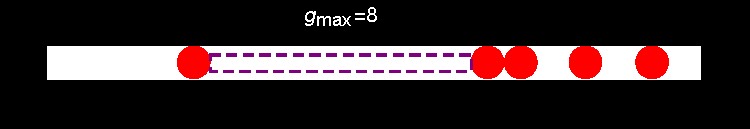
\includegraphics[width=1.0\columnwidth]{MaxGapm20n5s1.pdf}
\end{center}
\caption{\label{fig:coverage1d}
Exploring a 1D environment of size $m$ with $n$ robots.  Here $m=20$ and $n=5$.
}
\end{figure}


The expected number of moves for one robot to cover a 1D area of length $m$ is 
\begin{align}
\frac{1}{m} \sum _{i=1}^m (i+m) &= \frac{3 m+1}{2}  \label{eq:expectedMoves1robot1D}
\end{align}


If $n$ robots are uniformly distributed from $[1, m]$, as shown in Fig. \ref{fig:coverage1d}, the number of moves to discover the left and right boundaries is bounded by the maximum and minimum robots $ \pmin =\min(\mathbf{p})$, $\pmax =\max(\mathbf{p})$, requiring moving left $\pmin$, followed by a move of $m-(\pmax - \pmin ) $ right.
When $n=m$, the algorithm requires 2 moves, one left, one right.
The minimum time with $n\in[2,m-1]$ occurs with $\pmin$ at 1 and the $\pmax$ at $m$, requiring 3 moves, 1 left followed by 2 moves to the right.  

The maximum $2(m-n+1)$ occurs when the robots are arranged from $m-n$ to $m$, requiring $m-n+1$ moves to the left, followed by $m-n+1$ moves to the right.

This is drawing without replacement $n$ times from the set $[1, m]$.  The minimum is distributed between 1 and $m-n$, the maximum is distributed between $n$ and $m$.

The expected number of moves to reach both boundaries for $n$ robots in 1D is 
\begin{align}
\frac{1}{{m \choose n}} \sum_{\pmin = 1}^{m-n+1}  \sum_{\pmax = \pmin +n-1}^{m}   {\pmax -\pmin-1 \choose n-2} \left( 2 \pmin +m- \pmax +1\right)  \nonumber \\
= \frac{3(1+m)}{1+n}\label{eq:expectedMoveskrobots1D}
\end{align}

To fully \emph{cover} the area from 1 to $m$ requires that every position from 1 to $m$ be visited by at least one particle.  This time is dominated by the maximum gap $\overline{g}$. The total number of moves is then $ 2 \pmin +m- \pmax +1 + \max \left( \overline{g} - \left(\pmin + m-\pmax \right),0 \right)$.


 If all the particles are unit size, there are $m-n$ spaces, and these can be located before, between, or after the $n$ particles in $n+1$ locations giving ${m-n \choose n+1}$ possible configurations. The largest gap can be calculated exactly using a recurrence equation \citep{reviriego2011expected}, but a tight bound when
$m>n \log{n}$ is $\frac{m-n}{n+1} + \Theta \left( \sqrt{\frac{ (m-n)\log(n+1)}{n+1}} \right)$\citep{Raab1998}. 

\todo{I want an analytical result for the expected maximum gap. An analytical result for the maximum gap is given in \url{http://www.nebrija.es/~jmaestro/esa/papers/JDA2011.pdf}, but I have been unable to solve the coefficients in equation (18).  The same result is also in Section 9.4 of An Introduction to the Analysis of Algorithms, Second Edition by Robert Sedgewick and Philippe Flajolet, which I have ordered but don't have yet. -Aaron}


%\subsubsection{German tank problem}
%With multiple samples it is now possible to guess which direction is closer to the edge?  The population maximum is 
%uniformly minimum-variance unbiased estimator "The sample maximum plus the average gap between observations in the sample" --> but this will give the same distance to each side.  

\subsection{Mapping in 2D}

Not sure how to do this.  We have experiments.  There are so many options for arranging the freespace.  

The minimum time is a rectangle $k$ units tall and $N/k$ wide, with the robots arranged along the left wall. 1 move left registers the left wall, repeating $N/k$ moves up and right to find the top boundary and the right boundary,  followed by $N/k -1$ moves down and left to find the bottom boundary, with one final move down to register the furthest left bottom boundary.  This is 4(N/k) moves. %1+2(N/K) + 2(N/k -1)+1 = 

%Better if robots are in a square with side $\sqrt{N}$ and are in a vertical column spaced $\sqrt{N}/k-1$ apart.  moving left, followed by moving

What is the worst case?  


\subsection{Mapping in 3D}


We can do some experiments for this.  Perhaps draw wireframes for free spaces, draw red and blue cubes for unknown.  
TODO: draw with red circles/spheres for robots.

Define the probability of any given combination $T= {m \choose n}^{-1}$.  

If $n+1 = m$ there is one gap of size $1$, and $n+1$ possible locations.
The maximum gap size is $m-n$, and this gap can be placed before or after any of the $n$  numbers, for a total of $n+1$ possible positions.




%%%%%%%%%%%%%%%
%%%%%%%%%%%%%%%

%%%%%%%%%%%%%%%%%%%%%%%%%%%%%%%%%%%%%%%%%%%%%%%%%%%%%%%%%%%
\section{Related Work}\label{sec:RelatedWork}
%%%%%%%%%%%%%%%%%%%%%%%%%%%%%%%%%%%%%%%%%%%%%%%%%%%%%%%%%%%

Coverage using one robot is a canonical robotics problem \cite{choset2001coverage}. It has been studied in-depth for many applications including lawn mowing, harvesting, floor cleaning, 3D printing, robotic painting, and others. 

Coverage means that the robot has passed within one robot radius of every location in the workspace. Coverage with a swarm of robots is a key ability for a range of applications because swarms have higher fault tolerance and reduced completion time. Correspondingly, it has been studied from a control-theoretic perspective in  both centralized and decentralized approaches. For examples of each, see  \cite{zheng2005multi} and \cite{wagner1999distributed}.
%where the coverage is performed in such a way that robots are not aware of each other's existence but always cover a cell that is a non-critical point which does not disconnect the graph. 

Previous methods focus mostly on extending single robot coverage techniques to multi-robot systems. Solving coverage for synchronous multi-robots using online coverage techniques such as the boustrophedon technique of subdividing the 2D space into cells as in \cite{latimer2002towards} focuses on moving the robot teams in unison until they identify obstacles in their path. 
Once that happens, the team divides into smaller teams that continue the search in the smaller cells. 
This method is similar to our particles in the sense that robots try to move in the same direction as long as possible, but in our problem of interest the particles always move in the same direction and do not subdivide the space.  
The frontier cells exploration mentioned in \cite{yamauchi1998frontier} is an algorithm that is highly expansive as target locations to explore are selected using information from each robot, not a shared global map.
 Many algorithms have been developed after this pioneering work, and it showed how algorithms for single robot could be expanded to multi-robot systems. 
 The explorative bias of the technique allows it to define target cells of high priority to explore.   

Fundamental problems of robot navigation in an unknown environment have also received a large amount of attention from the theoretical side.
The classic prototype is the {\em linear-search problem}, which was first proposed by Bellman \cite{B63} and, independently,
by Beck\cite{B64}: An (immobile) object is located on the real line at an unknown distance $D$ and in an unknown direction.
Because the time necessary for locating the object may be arbitrarily high (as the object may be hidden far
from the origin), a useful measure for the performance of a search strategy
is the {\em competitive ratio}: This is the supremum of the ratio
between the time the searcher actually travels and the time she would have
taken if she had known the hiding place. 
 The competitive ratio is
a standard notion in the context of online algorithms; see \cite{FW98}
for a comprehensive overview. 
For the linear-search problem, the optimal competitive ratio is 9,
as was first shown by Beck and Newman \cite{BN70} and generalized by Gal~\cite{G72,G74}: The search should alternate
between going to the right and to the left, at each iteration doubling
her step size. This can be extended to other scenarios: For the case in which changing direction during the course 
of the search incurs an additional cost of $d$, Demaine et al.~\cite{dfg-olstc-06} showed that an optimal strategy can 
locate an object with total cost $9D+2d$, which is optimal; see Arkin et al.~\cite{abd+-octtc-05} for the generalized
offline problem of covering with turn cost. Other related algorithmic work in an unknown setting includes Kao et al.~\cite{KRT96}
in a randomized setting, Baeza-Yates et al.~\cite{BCR93} for searching in the plane; for broad surveys on mathematical
methods, see the books by Gal~\cite{G80} and by Alpern and Gal~\cite{AG03}.
Of particular relevance for the content of this paper is 
Fekete et al.~\cite{fkn-sar-04,fkn-osar-06} for online searching by an autonomous robot in an unknown environment,
where both moving and measuring incur individual costs, and Fekete et al.~\cite{fms-mctc-10} for an (offline)
setting that studies the closely related bicriteria version of covering with travel cost.
For another recent work on mapping and coverage by a swarm of robot with limited information and capabilities, see~\cite{lfm-stmrs-16}.

However, all these approaches assume a level of intelligence and autonomy in individual robots that exceeds the capabilities of many systems, including current micro- and nano-robots.  Current micro- and nano-robots, such as those in~\cite{Chowdhury2015,martel2015magnetotactic,Xiaohui2015magnetiteMicroswimmers} cannot have onboard computation. Thus, we will be referring to them as {\em particles}. For these reasons, this paper focuses on centralized techniques that apply the same control input to each member of a particle swarm.%In \cite{shahrokhi2016algorithms}, global control is used to shape a swarm and the convenience and mass is controlled to use swarms for high accuracy assembly. The algorithms showcased in this work show how environmental factors such as wall friction can be used to shape swarms. The usage of limited parameters to control a large swarm gives us insight into how planning must be approached for problems where large number of globally controlled robots must be used. By following the covariance of a swarm, we can see how dispersed a swarm is. This will be useful for us to determine how explorative our algorithms are, when searching the workspace.   
%Precision control requires breaking the symmetry caused by the global input.

%Symmetry can be broken using agents that respond differently to the global control, either through agent-agent reactions, see work modeling biological swarms \cite{bertozzi2015ring}, or engineered inhomogeneity  \cite{Donald2013,bretl2007,beckerIJRR2014}.
%This work assumes a uniform control with homogenous agents, as in~\cite{Becker2013b}. 


%%%%%%%%%%%%%%%
%%%%%%%%%%%%%%%%%%%%%%%%%%%%%%%%%%%%%%%%%%%%%%%%%%%%%%%%%%%
\section{Theory}
\label{sec:theory}
%%%%%%%%%%%%%%%%%%%%%%%%%%%%%%%%%%%%%%%%%%%%%%%%%%%%%%%%%%%
This section examines the problem of mapping with uniform inputs in 1 and 2 dimensions. For ease of exposition this section represents workspaces as discretised regions. Future work should extend this to continuous regions.
 
\subsection{Mapping in 1D}
We begin with the single particle case, then proceed to the $n$ particle case. 
\subsubsection{1D mapping with 1 particle}
A particle is initialized uniformly randomly in a linear free-space $m$ units wide.  To \emph{map} this region the particle needs to choose one direction, move until it hits a boundary, and then switch direction and move until it reaches the other boundary.


Without loss of generality, assume the particle always starts going left, and label the free-space from 1 to $m$ left to right.  If the initial position is 1, the particle tries to move 1 unit to the left, but is stopped by the boundary. The particle then moves $m-1$ moves to the right.  The final $m^{\textrm{th}}$ move right results in a collision with the right wall, and thus mapping requires $m+1$ moves. This is the minimum number of moves.  The worst case is if the particle starts at $m$, requiring $2m$ moves: $m$ moves to the left and $m$ moves to the right.

The expected number of moves for one particle to cover a 1D area of length $m$ is 
\begin{align}
\frac{1}{m} \sum _{i=1}^m (i+m) &= \frac{3 m+1}{2}  \label{eq:expectedMoves1particle1D}
\end{align}

\subsubsection{1D mapping with n particles}

\begin{figure}
\begin{center}
	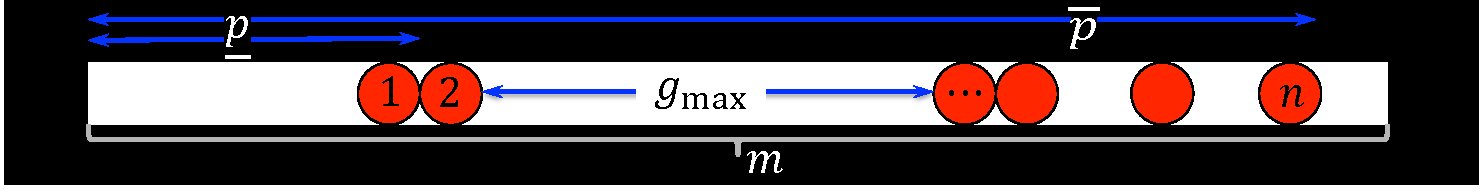
\includegraphics[width=1.0\columnwidth]{MaxGapm20n5s1v3.pdf}
\end{center}
\caption{\label{fig:coverage1d}
Exploring a 1D environment of size $m$ with $n$ particles of unit size. Here $m=20$ and $n=6$. $\pmin=4$, $\pmax=19$ and $g_{max}= 7$
}
\end{figure}

For $n>1$ the average expected number of moves is calculated as follows.
Let $\mathbf{p}$ be the list of positions of $n$ unit size particles uniformly distributed from $[1, m]$.
As shown in Fig. \ref{fig:coverage1d}, the number of moves to discover the left and right boundaries is bounded by the maximum and minimum particles $ \pmin =\min(\mathbf{p})$, $\pmax =\max(\mathbf{p})$, requiring moving left $\pmin$, followed by a move of $m-(\pmax - \pmin )+1 $ right.
When $n=m$, the algorithm requires 2 moves, one left, one right.
The minimum time with $n\in[2,m-1]$ occurs with $\pmin$ at 1 and $\pmax$ at $m$, requiring 3 moves, 1 left followed by 2 moves to the right.  

The maximum $2(m-n+1)$ occurs when the particles are arranged from $m-n$ to $m$, requiring $m-n+1$ moves to the left, followed by $m-n+1$ moves to the right.

This is drawing without replacement $n$ times from the set $[1, m]$.  The minimum is distributed between 1 and $m-n$, the maximum is distributed between $n$ and $m$.

The expected number of moves to reach both boundaries for $n$ particles in 1D is 

\begin{align}
{\scriptstyle \frac{1}{{m \choose n}} \sum_{\pmin = 1}^{m-n+1}  \sum_{\pmax = \pmin +n-1}^{m}   {\pmax -\pmin-1 \choose n-2} \left( 2 \pmin +m- \pmax +1\right)-\frac{\left(m-n+1\right)}{{m \choose n}}} \nonumber
\\= \frac{3(1+m)}{1+n} - \frac{\left(m-n+1\right)}{{m \choose n}}
\label{eq:expectedMoveskparticles1D}
 \end{align}

This reduces to Eqn.~\eqref{eq:expectedMoves1particle1D} when $n=1$. To fully map the area from 1 to $m$ requires that every position from 1 to $m$ be visited by at least one particle. This time is dominated by the maximum gap $\overline{g}$. The total number of moves is then $ 2 \pmin +m- \pmax +1 + \max \left( \overline{g} - \left(\pmin + m-\pmax \right),0 \right)$.


 Since these particles are unit size, there are $m-n$ spaces, and these can be located before, between, or after the $n$ particles in $n+1$ locations giving ${m-n \choose n+1}$ possible configurations. The largest gap can be calculated exactly using a recurrence equation \cite{reviriego2011expected}, but a tight bound when
$m>n \log{n}$ is $\frac{m-n}{n+1} + \Theta \left( \sqrt{\frac{ (m-n)\log(n+1)}{n+1}} \right)$\cite{Raab1998}. 

%\todo{I want an analytical result for the expected maximum gap. An analytical result for the maximum gap is given in \url{http://www.nebrija.es/~jmaestro/esa/papers/JDA2011.pdf}, but I have been unable to solve the coefficients in equation (18).  The same result is also in Section 9.4 of An Introduction to the Analysis of Algorithms, Second Edition by Robert Sedgewick and Philippe Flajolet, which I have ordered but don't have yet. -Aaron}
%Define the probability of any given combination $T= {m \choose n}^{-1}$.  
%If $n+1 = m$ there is one gap of size $1$, and $n+1$ possible locations.
%The maximum gap size is $m-n$, and this gap can be placed before or after any of the $n$  numbers, for a total of $n+1$ possible positions.


\subsubsection{1D mapping with scan and move costs}
 Often scanning (imaging) and moving the particles costs time and energy.
 When controlling particles with MRI as in \cite{chanu2008adapting}, the MRI machine iterates between imaging and applying gradient forces to move the particles.
 This section examines 1D mapping when scanning the workspace and moving the particles a unit distance have associated costs. 
The objective is to minimize a linear combination of costs for moving and measuring; however, the precise respective coefficients may be subject
to change, or even unknown in advance turning this into a {\em bicriteria problem}, in which both parameters need to be within 
a bounded ratio of those in an optimal solution. For simpler notation, we write $(a,b)$ for a schedule that involves $a$ unit steps and $b$ scans.

For a more detailed analysis, assume that the left boundary is located $D$ units to the left of the leftmost particle.
(This analysis can be applied in both directions.)
The theoretically optimal, yet elusive, solution requires scanning the workspace to map particle locations,
moving $D+1$ units to the left, 
then scanning to detect that the leftmost particle has only moved $D$ units and thus has encountered the wall,
for a total cost of $(D+1,2)$ for the schedule.

We can achieve a schedule with $D+1$ steps by scanning after each step, for a total cost of $(D+1,D+2)$;
while this is optimal with respect to steps, the involved scan cost is large compared to the optimum.
At the expense of increasing the number of steps we can reduce the number of scans by successively doubling the number 
of steps between scans, i.e., performing the $i^{\textrm{th}}$ scan after $2^i$ steps, resulting in total cost at most $(2D+2,\log_2 D)$; replacing
the base of $2$ by an arbitrary constant $k$, we get $(k\times(D+1), \log_k D)$. This is within a constant of the optimal. 
On the other hand, moving a sufficiently large number $M$ of steps (known to satisfy $M\geq D$) before performing the second 
scan yields $(M,2)$, which is optimal with respect to scan cost, but bad in terms of the cost for motion.

Balancing the competitive factor for both parameters can be achieved as follows:
perform the $i$th scan at position $i^i$. This yields a simultaneous competitive factor of $O(\log D/\log\log D)$ for {\em both} parameters.

\begin{theorem}
\label{th:eyetoeye}
The hyperexponential search sequence $i^i$ yields a best possible simultaneous competitive factor of $O(\log D/\log\log D)$ for {\em both} parameters
of the bicriteria search problem.
\end{theorem}

\begin{proof}
Let us first consider the number of scans.
If the boundary is properly detected in step $j+1$, the particle must have encountered it between steps $j$ and $j+1$, i.e. $j^j \leq D < (j+1)^{j+1}$.
Now we can employ the Lambert $W$ function, which is the inverse function of $f(x)=xe^x$; note that 
$$\log x = W(\log x) \cdot e^{W(\log x)},$$ 
so
	$$\log \log x = (\log W(\log x) + W(\log x)),$$
and therefore
	$$W(\log x) \in \Theta(\log \log x).$$

This implies that $j\leq \log D/ W(\log D)$ (the inverse of $j^j$), hence $\Theta(\log D/ \log\log D)+1$ scans have been made, while the optimum are $2$ scans.

The moved distance is $(j+1)^{j+1}$, while the optimum is $D\geq j^j$.
Hence, we get the ratio 
\begin{align}
\frac{(j+1)^{(j+1)}}{j^j}=(j+1)\frac{(j+1)^j}{j^j},\label{eq:MoveDistanceRatio}
\end{align}
 where $0\leq \frac{(j+1)^j}{j^j}\leq \mathrm{e}$ for $j>0$.
 
Because $j\leq \log D/ W(\log D)$, we obtain 
\begin{align}
\frac{(j+1)^{(j+1)}}{j^j}\leq \mathrm{e}\frac{\log n}{ W(\log n)}+\mathrm{e}\label{eq:MoveDistanceRatioInequality}
\end{align}
 for $j>0$. Clearly, this is again in within a factor of $\Theta(\log D/ \log\log D)$ of the optimum.
 
 To see that this balanced factor is best possible, observe that $\left(\frac{\log D}{\log\log D}\right)^{\left(\frac{\log D}{\log\log D}\right)}\in \Theta(D)$, with the base corresponding to the ratio between step lengths and the exponent to the number of scans. Therefore, using significantly fewer than $\log D/ \log\log D$ scans would require increasing the base, yielding a worse competitive factor for the step length; on the other hand, decreasing the base in order to decrease the competitive factor for the step length would require increasing the exponent, yielding a worse competitive factor for the scan cost.
\end{proof}

%\subsubsection{German tank problem}
%With multiple samples it is now possible to guess which direction is closer to the edge?  The population maximum is 
%uniformly minimum-variance unbiased estimator "The sample maximum plus the average gap between observations in the sample" --> but this will give the same distance to each side.  

\subsection{Mapping in 2D}


\subsubsection{2D mapping with 1 particle}
The shortest path for mapping with 1 particle is a version of depth-first search that halts when all frontier cells have been explored.
As long as the all the free cells are connected, depth-first-search (DFS) is the optimal solution to mapping.
%\todo{Q2.Domink --- Prove that DFS is the optimal solution with 1 particle }
%<Dominik> <- this tag is just to ease possible merges. Feel free to edit or delete.
Even if the environment is known in advance, the problem is NP-hard as can be shown by a trivial reduction to Hamiltonian paths in grid graphs \cite{itai1982hamilton}. %NP-hardness shown in Itai, Alon, Christos H. Papadimitriou, and Jayme Luiz Szwarcfiter. "Hamilton paths in grid graphs." SIAM Journal on Computing 11.4 (1982): 676-686.
One can easily show that a simple DFS guarantees a competitive ratio of $2$: the depth-first tree has $m-1$ edges and each edge is traversed at most twice. 
Any path that covers $m$ cells needs to traverse least $m-1$ edges, and hence the depth-first-search is at most twice as long as an optimal coverage path.

For showing that no algorithm can perform better one needs only a simple 1-dimensional graph that goes to the left and to the right.
If the algorithm chooses to go arbitrarily to one side, we can make it do a long walk of length $m$ and then return it just for a single field on the other side ($2m+1$ vs.\ $2+m$).
If the algorithm decides to switch the direction after some time after arbitrary zig-zags (of increasing cost) of cost $z$ (center to one side to other side) we decide that there is a single field on both sides.
The algorithm now needs to go one additional time from one side to the other and back (cost $>z$) while the optimum cost would have been $\leq z+3$.
If the algorithm switches from the second form to the first, the first argument still applies.

%TOURS (related work, actually doesn't belong here but you probably find it here most easily. Just to help with related work.):
Most previous work on grid graph exploration focused on exploration tours, i.e., after exploration one has to go back to the start position.
If the environment is known in advance, this equals the traveling salesman problem and a polynomial-time approximation scheme is known~\cite{klein2008linear}. % Philip N. Klein.  A linear-time approximation scheme for TSP in undirected  planar  graphs  with  edge-weights.  SIAM  Journal  on  Computing , 37(6):1926–1952, 2008.
If the environment is unknown, as it is in our case, the best achievable competitive ratio is $2$ in general grid graphs (achieved by depth first search) and $7/6$ for simple grid graphs ($4/3$ achieved by smartDFS \cite{icking2005exploring}). %Icking et al. http://link.springer.com/chapter/10.1007/11533719_53 http://www.geometrylab.de/applet-55
%</Dominik>

\subsubsection{2D mapping with $n$ particles}

Another problem with this type of mapping is identifying which move sequence guarantees the shortest path in the worst case.
%At the beginning there can be at most four frontier cells per particle to be explored. 
 %As the particles begin to move, the number of frontier cells explored and the number of free cells identified increases. 
 
 We describe three algorithms of increasing complexity for 2D mapping.
 If we implement a random move algorithm as described in {\sc RandomMoves}, at each step the particles all move in the same randomly selected direction until there are no frontier cells left on the map. 
 \emph{MoveType} is a vector that holds the four possible move types. 
 The map $\mathbf{M}$ is a matrix the size of the work space. 
 Each cell of  $\mathbf{M}$ holds one of five values that denote: \emph{Particle}, \emph{Frontier}, \emph{Unknown}, \emph{Freespace} and \emph{Obstacle}. 
 At each step {\sc Frontier} returns the locations of frontier cells in $\mathbf{M}$ and $\mathbf{r}$ has the list of particle locations.
 The \emph{move} is implemented to update the map $\mathbf{M}$ and the particle locations $\mathbf{r}$ by calling {\sc Move\&\!Update}. 
{\sc RandomMoves} requires minimal computation and is probabilistically complete, so eventually the swarm maps the free cells~\cite{kahn1989cover}. 
 However, this method of mapping is inefficient, resulting in long mapping times, especially with small numbers of particles in large, torturous maps with many turns. 

  \begin{algorithm}
\caption{\sc RandomMoves($\mathbf{M},\mathbf{r}$)   \label{alg:randommove}}
\begin{algorithmic}[1]
\State \emph{MoveType}$ = \{l,r,u,d\}$ 
\While{$|${\sc Frontier}$(\mathbf{M})| >0  $}
%\While{ $|\mathbf{M}.Frontiercells| >0  $}
\State \emph{move} $ \gets$ {\sc random}$($\emph{MoveType}$)$
\State $\{\mathbf{M}, \mathbf{r}\} \gets ${\sc Move\&\!Update}$(move, \mathbf{M}, \mathbf{r}) $
\EndWhile
\end{algorithmic}
\end{algorithm}

A better way to map the world is to deliberately move particles toward frontier cells. 
We could choose one particle as the $elect$ particle and perform motion planning using this particle. 
In {\sc ElectParticle}, one of the particles is selected as \emph{elect}. 
As long as the number of frontiers to be visited is at least one, the algorithm proceeds by generating a $mvSq$ from the current position of the elect particle to the nearest frontier cell. 
The \emph{mvSq} is generated by a breadth-first-search (BFS) shortest path algorithm which requires the map $\mathbf{M}$, source \emph{elect}, and the cells {\sc Frontier}$(\mathbf{M})$. A representative $mvSq$ is $\langle u,r,d,d,r,u,\ldots\rangle$. 
The list of moves in \emph{mvSq} are implemented by iteratively calling the {\sc Move\&\!Update} function for the length of $mvSq$. 


{\sc ElectParticle} will explore the target frontier cell by the end of $mvSq$. 
However, often with large-population swarms the whole $mvSq$ need not be implemented. 
Every time {\sc Move\&\!Update} is called, the nearest frontier is updated and $mvSq$ is also updated because as the particles start to move, the target frontier cell  might be explored by a non-elect  particle. 

 {\sc ClosestFrontier} exploits this fact by computing a BFS shortest path from all particles to all frontier cells.   
  \begin{algorithm}
\caption{\sc ElectParticle($\mathbf{M},\mathbf{r}$)   \label{alg:ElectParticle}}
\begin{algorithmic}[1] 
\State \emph{elect} $ \gets$ {\sc random}$(\mathbf{r})$
\While{$|${\sc Frontier}$(\mathbf{M})| >0  $}
\State \emph{mvSq} $ \gets$ BFS$(\mathbf{M},$\emph{elect}$,${\sc Frontier}$(\mathbf{M}))$
\For { \emph{iter} $:=1$ $\mathbf{ to}$ $|$\emph{mvSq}$| $ $\mathbf{ step }$ $ 1$} 
\State $\{\mathbf{M}, $\emph{elect}$\} \gets ${\sc Move\&\!Update}$($\emph{mvSq}$, \mathbf{M}, $\emph{elect}$) $
 \EndFor
\EndWhile
\end{algorithmic}
\end{algorithm}

In each loop of {\sc ClosestFrontier}, all the moves in $mvSq$ are implemented to explore the target frontier cell since it is the shortest possible route to a frontier cell. 
At time 0, there will be at most 4$n$ equally valid destinations that can be visited since cells to the side of each particle not neighboring another particle are frontier cells. 
%Our BFS expands the search in order, ${l,r,u,d}$, so the first move is $l$. 
Each $mvSq$ guarantees classification of one frontier cell into obstacle or free space.
When a frontier cell is explored it is labeled either free or obstacle. There can be a net gain of at most two frontier cells per particle that encounters a free cell or no new frontier cells if the frontier cell contained an obstacle. 

 
The simulation results in Section \ref{sec:simulation} show that both map complexity and distribution affect the number of moves taken to map the work space. {\sc RandomMove} uses no information from the data except for checking completion. {\sc ElectParticle} uses the location and distance data from one particle to map the work space. {\sc ClosestFrontier} improves the performance of mapping by using all the data. 

  \begin{algorithm}
\caption{\sc ClosestFrontier($\mathbf{M},\mathbf{r}$) \label{alg:ClosestFrontier}}
\begin{algorithmic}[1]
\While{$|${\sc Frontier}$(\mathbf{M})| >0  $}
\State$mvSq \gets$ BFS$(\mathbf{M},\mathbf{r},${\sc Frontier}$(\mathbf{M}))$
\For {$iter:=1$ $\mathbf{ to}$ $|mvSq| $ $\mathbf{ step }$ $ 1$}  
\State $\{\mathbf{M},\mathbf{r}\} \gets ${\sc Move\&\!Update}$(mvSq, \mathbf{M}, \mathbf{r}) $

 \EndFor
  
\EndWhile
\end{algorithmic}
\end{algorithm}
%<Dominik>
 %Comment: Just some quick text because this section is still missing. Feel free to remove or change.
While {\sc ClosestFrontier} is usually the more reasonable approach in practice than DFS with a single particle, we are only able to show a trivial weaker bound on the corresponding moves. {\sc ClosestFrontier} is not optimal. It can need $\Omega(n^2)$ moves while an optimal strategy only needs $O(n)$.
An example can be seen in Fig.~\ref{fig:square-worse-than-opt}.
In some scenarios {\sc ClosestFrontier} can perform worse than DFS with a single particle, e.g., in Fig.~\ref{fig:greed-worse-than-dfs}.



\begin{figure}
\begin{center}
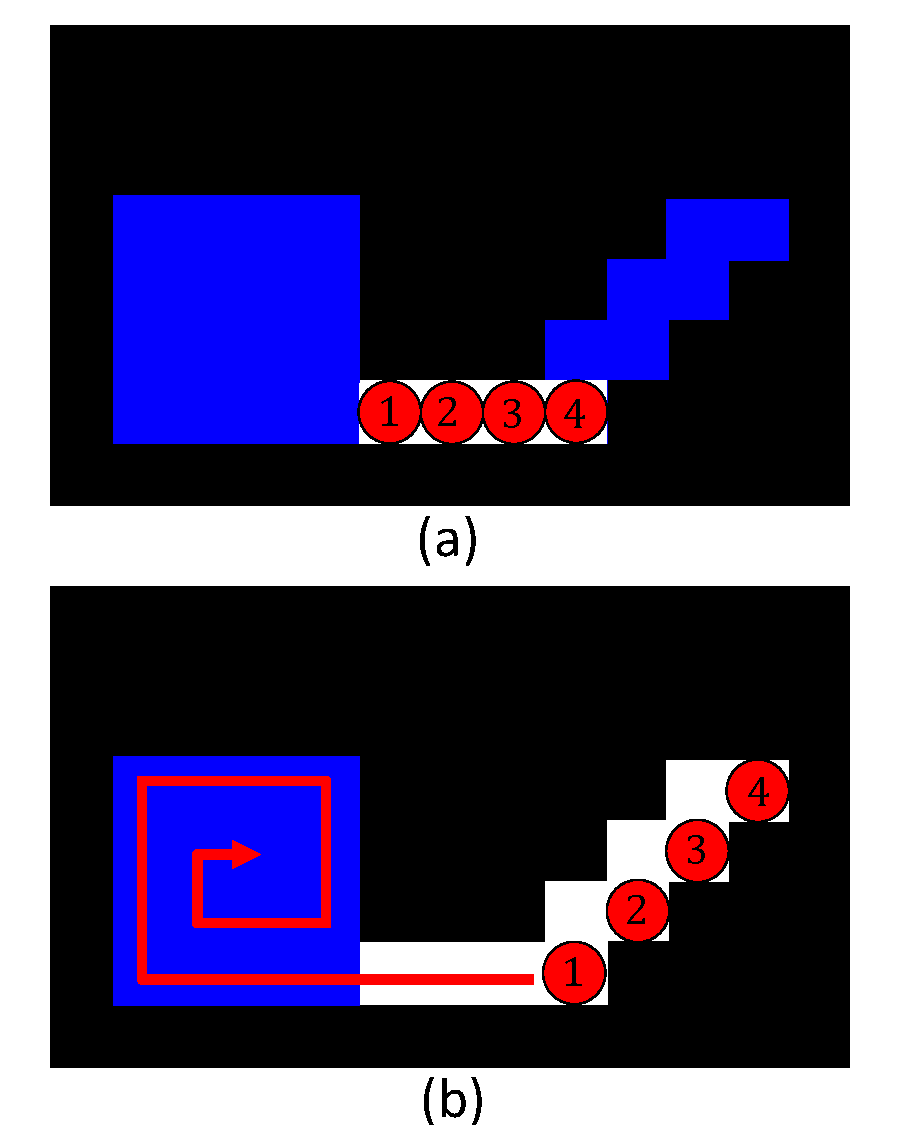
\includegraphics[width=1.0\columnwidth]{greedy2}
\end{center}
\caption{\label{fig:square-worse-than-opt}
{\sc ClosestFrontier} is not optimal in all cases. {\sc ClosestFrontier}, which is greedy, could go right first and then cover the square with a single particle which takes $\Omega(n^2)$ moves while the optimal solution, which visits the square in parallel using all $n$ particles, only needs $O(n)$ moves.}
\end{figure}
	
\begin{figure}
\begin{center}	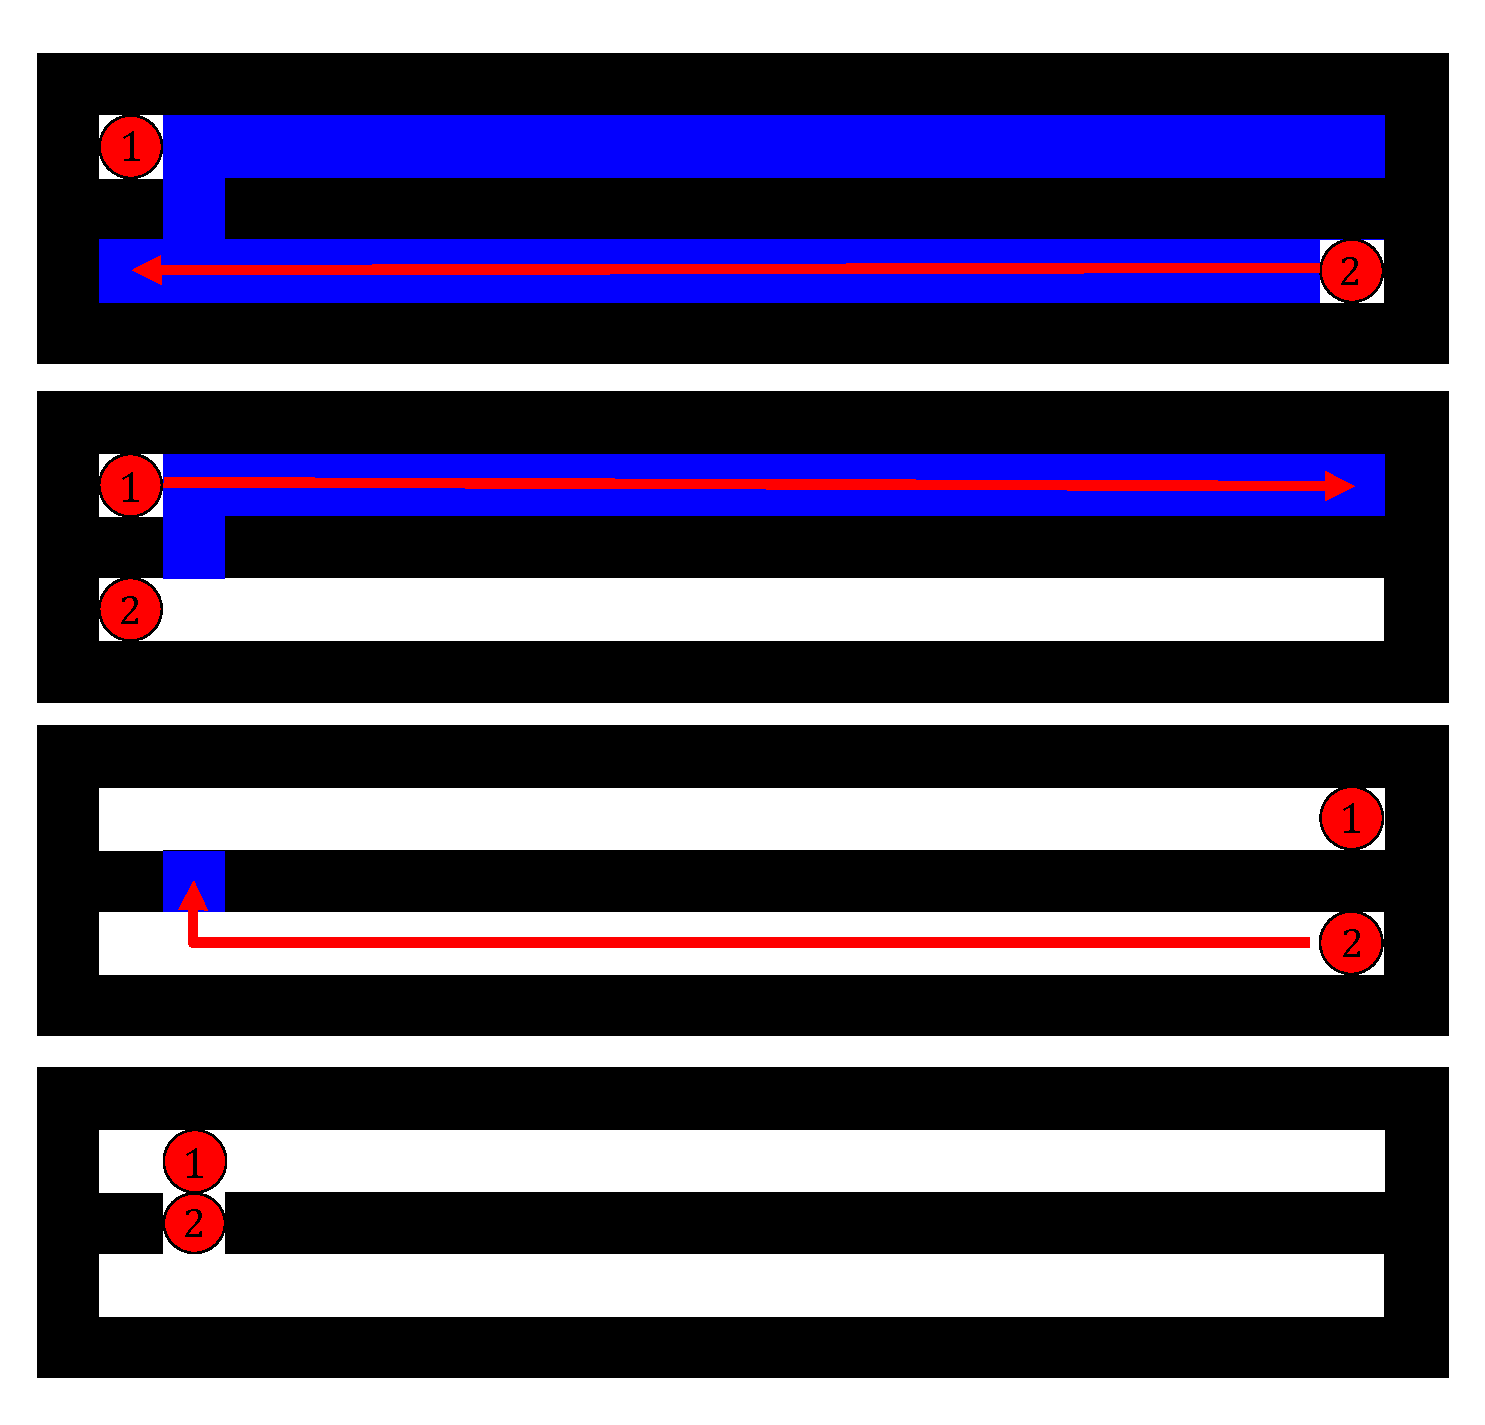
\includegraphics[width=0.8\columnwidth]{greedy1}
\end{center}
\caption{\label{fig:greed-worse-than-dfs}
{\sc ClosestFrontier} can be worse than DFS in some cases as well. In this example, using {\sc ClosestFrontier} is $1.5\times$ worse than DFS using only particle 2.}
%If the move preference order is $\{l,u,r,d\}$ using Alg.~\ref{alg:ClosestFrontier}. then coverage with two particles takes approximately 1.5 times longer than with just the bottom right particle.
\end{figure}

%\begin{figure}
%	\centering
%	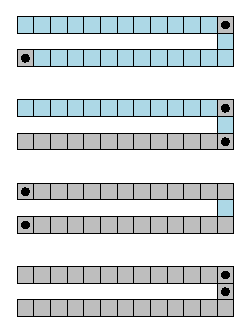
\includegraphics[width=0.2\textwidth]{greedy-worse-than-dfs.eps}
%	\caption{In this example, the greedy strategy is $1.5\times$ worse than DFS with the bottom left particle.}
%	\label{fig:greed-worse-than-dfs}
%\end{figure}
%TRIVIAL UPPER BOUND
\begin{theorem}
	{\sc ClosestFrontier} needs at most $O(m^2)$ moves where $m$ is the number of cells. 
\end{theorem}
\begin{proof}
	The distance between a particle and the closest frontier cell can be at most the number of all already visited cells.
	Hence, the distance for visiting the $i^{\textrm{th}}$ field is bounded by $i$.
	The overall number of moves is bounded by $\sum_{i=1,\ldots,m} i = 0.5\cdot m\cdot (m+1)$.
\end{proof}
%</Dominik>

%\todo{insert plot of boundary nodes as a function of moves for 3 different values of no. of particles. n=100, n=500 and n=2000} 



%Better if particles are in a square with side $\sqrt{N}$ and are in a vertical column spaced $\sqrt{N}/k-1$ apart.  moving left, followed by moving
%<Dominik>
%Comment: Just some quick text because this section is still missing. Feel free to remove or change.


%\begin{figure}
%	\centering
%	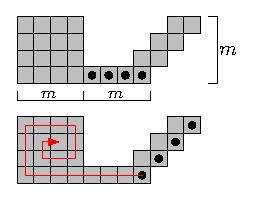
\includegraphics[width=0.2\textwidth]{square-bad-case.eps}
%	\caption{If the move preference is counter clockwise, the greedy strategy might selects to go right and then covers the square with a single particle which takes $\Omega(m^2)$ moves while the optimal strategy that visits the square in parallel with the $m$ particles, only needs $O(m)$ moves.}
%	\label{fig:square-worse-than-opt}
%\end{figure}
%</Dominik>

%\todo{Q4.What is the complexity of the 2D problem? 
%NP-hard already for 1-particle, see previous section. The decision problem is NP-complete (i.e., it's not worse than NP-hard). %Dominik
%}

%\todo{Q5.Can we do better than the greedy algorithm for 2D coverage?  }

%\todo{Q6.What is the running time for the greedy algorithm?  }
%<Dominik>
%Comment: Just some quick text because this section is still missing. Feel free to remove or change.
\begin{theorem}
	{\sc ClosestFrontier} has a computational complexity in $O(m^2)$.
\end{theorem}
\begin{proof}
	For an environment with $m$ cells, there are at most $m$ iterations.
	Since the edges in the grid graph are not weighted and each cell only has at most four neighbors, the shortest path from a particle to the frontier cell can be calculated in $O(m)$ time by a simple breadth first search.
	%NOTE: CURRENTLY USING DIJKSTRA WHICH HAS A HIGHER COMPLEXITY.
\end{proof}
%</Dominik>

%Completion time is a function of the initial particle distribution. The minimum mapping time for a rectangle $n$ units tall and $m/n$ wide, with the $n$ particles arranged along the left wall. 1 move left registers the left wall, repeating $m/n$ moves up, down, and right to find the top and bottom boundaries and move right until reaching the right boundary.  This requires $3(m/n)+1$ moves. %1+2(N/K) + 2(N/k -1)+1 = 

%Better if particles are in a square with side $\sqrt{N}$ and are in a vertical column spaced $\sqrt{N}/k-1$ apart.  moving left, followed by moving
Finally, completion time is also a function of the map geometry.
Mapping requires exploring all the free spaces and the boundary of the free spaces.
The number of map cells that need to be explored is the \emph{Area} $+$ \emph{Perimeter} $-~n$. 
This is minimized by a circular region and maximized by a linear region.
 For example,  a linear region has $m+(2m+2)-n$ cells to explore, while a 
 square region has $m + (4 \sqrt{m}) -n$ cells to explore.

%a $5\times4$ rectangular grid, then the number of map cells that need to be classified is only $a\cdot b+2(a+b)-n=33$ where $a=5$ and $b=4$.  
%  Fig.~\ref{fig:greedy1} shows a scenario where two particles perform worse than one particle. 
 % Here for $m$=43, it takes the two particles 60 moves to complete coverage whereas if particle 2 alone is present, it would take 44 moves. 
 % This shows that particle distribution is key to determining the number of moves taken. This behavior is also seen in the simulation experiment in Sec.~\ref{sec:simulation}. 
%  But in general, for a uniform random spread of particles the algorithm works better on an average with a small standard deviation.





%\subsection{Mapping in 3D}

%\todo{We can do some experiments for this.  Perhaps draw wireframes for free spaces, draw red and blue cubes for unknown.  TODO: draw with red circles/spheres for particles.}






%%%%%%%%%%%%%%%
%%%%%%%%%%%%%%%

\section{Simulation}\label{sec:simulation}


\subsection{1D mapping}

  \begin{figure}
\begin{center}
	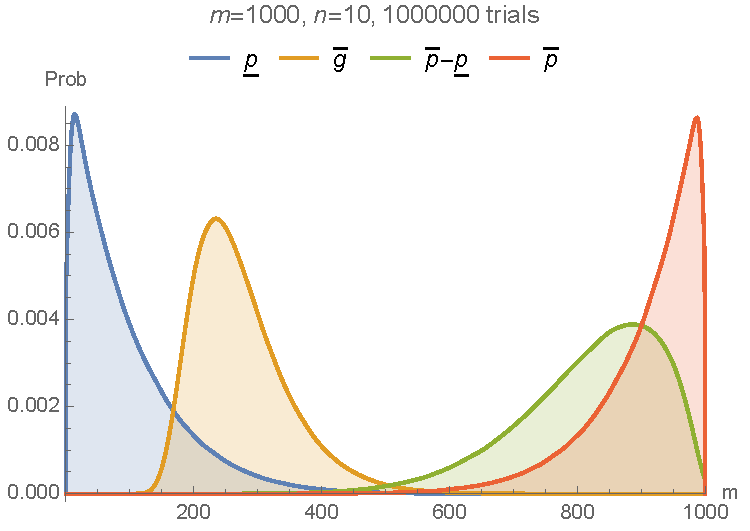
\includegraphics[width=1.0\columnwidth]{Prob1DcoverageGaps}
\end{center}
\caption{\label{fig:Prob1DcoverageGaps}
With a connected, 1D freespace $m$ = 1000 and $n=10$ particles, the distributions for the gap before the first $\overline{p}$ and after the last $\underline{p}$  gaps are symmetric. The maximum gap $\overline{g} \approx 250$.}
\end{figure}

\begin{figure}
\begin{center}
	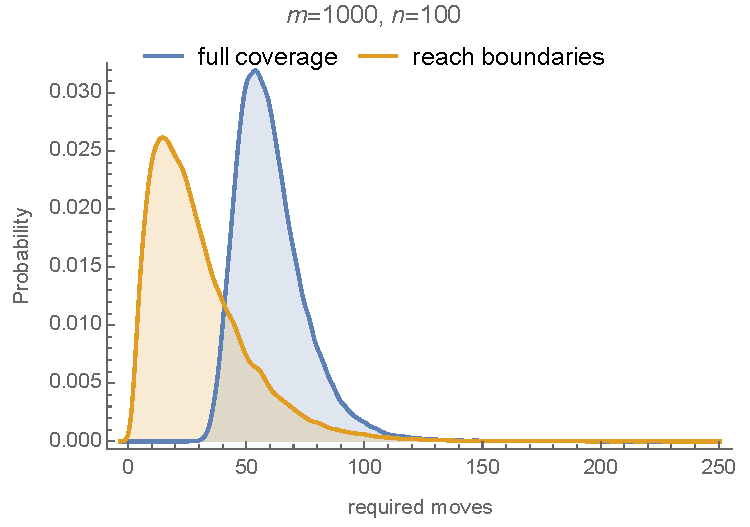
\includegraphics[width=1.0\columnwidth]{SimReachBoundaryCoverage}
\end{center}
\caption{\label{fig:SimReachBoundaryCoverage}
Full coverage in 1D with $m$ = 1000 and $n=10$ particles requires 60.7 moves on average, while reaching the boundaries requires only 29.8.}
\end{figure}

  
 1D simulations were conducted in Mathematica, with code available at \cite{Arun2017GitHubUniformMapping}. 
 Fig.~\ref{fig:Prob1DcoverageGaps} shows the distributions for the minimum and maximum initial particle locations $\underline{p}$ and $\overline{p}$, the maximum gap $\overline{g}$, and the spread between the minimum and maximum $\overline{p}-\underline{p}$ for 1,000,000 Monte Carlo trials.
 The expected gap between the first particle and the boundary $\underline{p}$ is 90.94.
 The expected gap between the last particle and the boundary $\overline{p}$ is 90.98.
  The expected maximum gap is $\overline{g}$ is 273.9.
  
  Fig.~\ref{fig:SimReachBoundaryCoverage} shows that full coverage requires approximately twice the time required to explore the left and right boundaries when $m=1000$ and $n=100$.

  
  \subsection{2D mapping}  
2D simulations were conducted in Matlab, with code available at \cite{Arun2017matlabUniformMapping}. All simulations used maps with 5000 free cells.
  Each simulation trial was repeated 100 times.
  The number of particles ranged from 100 to 5000 by increments of 100.
  In each run except Fig.~\ref{fig:RegionvsFloodvsUniform} the particles were placed uniformly randomly throughout the workspace. 
  
 %%%%%%%%%%%%%%%  MappingAlg3maps
  The comparison plot Fig.~\ref{fig:MappingAlg3maps} between the mapping of  four 2D maps� \emph{H-tree}, \emph{complex}, \emph{empty rectangle} and \emph{linear} and a 1D map using the {\sc ClosestFrontier} algorithm, shows that the H-tree map requires the most moves because it has the highest number of turns. 
  In Fig.~\ref{fig:MappingAlg3maps} there is an observable difference in moves between the linear and rectangular workspaces. 
	One reason is because the perimeter of the linear map is much larger than the rectangular map. 
	The number of cells to explore is $3m+2 = 15,002$ for the linear map, but only $m + 2(50+100) = 5,300$ for the rectangular map. 
	Only when the number of particles is around 2/3 of the number of free spaces is there an overlap between the moves taken to map the rectangular space and the linear space. 

 
\begin{figure}
\begin{center}
	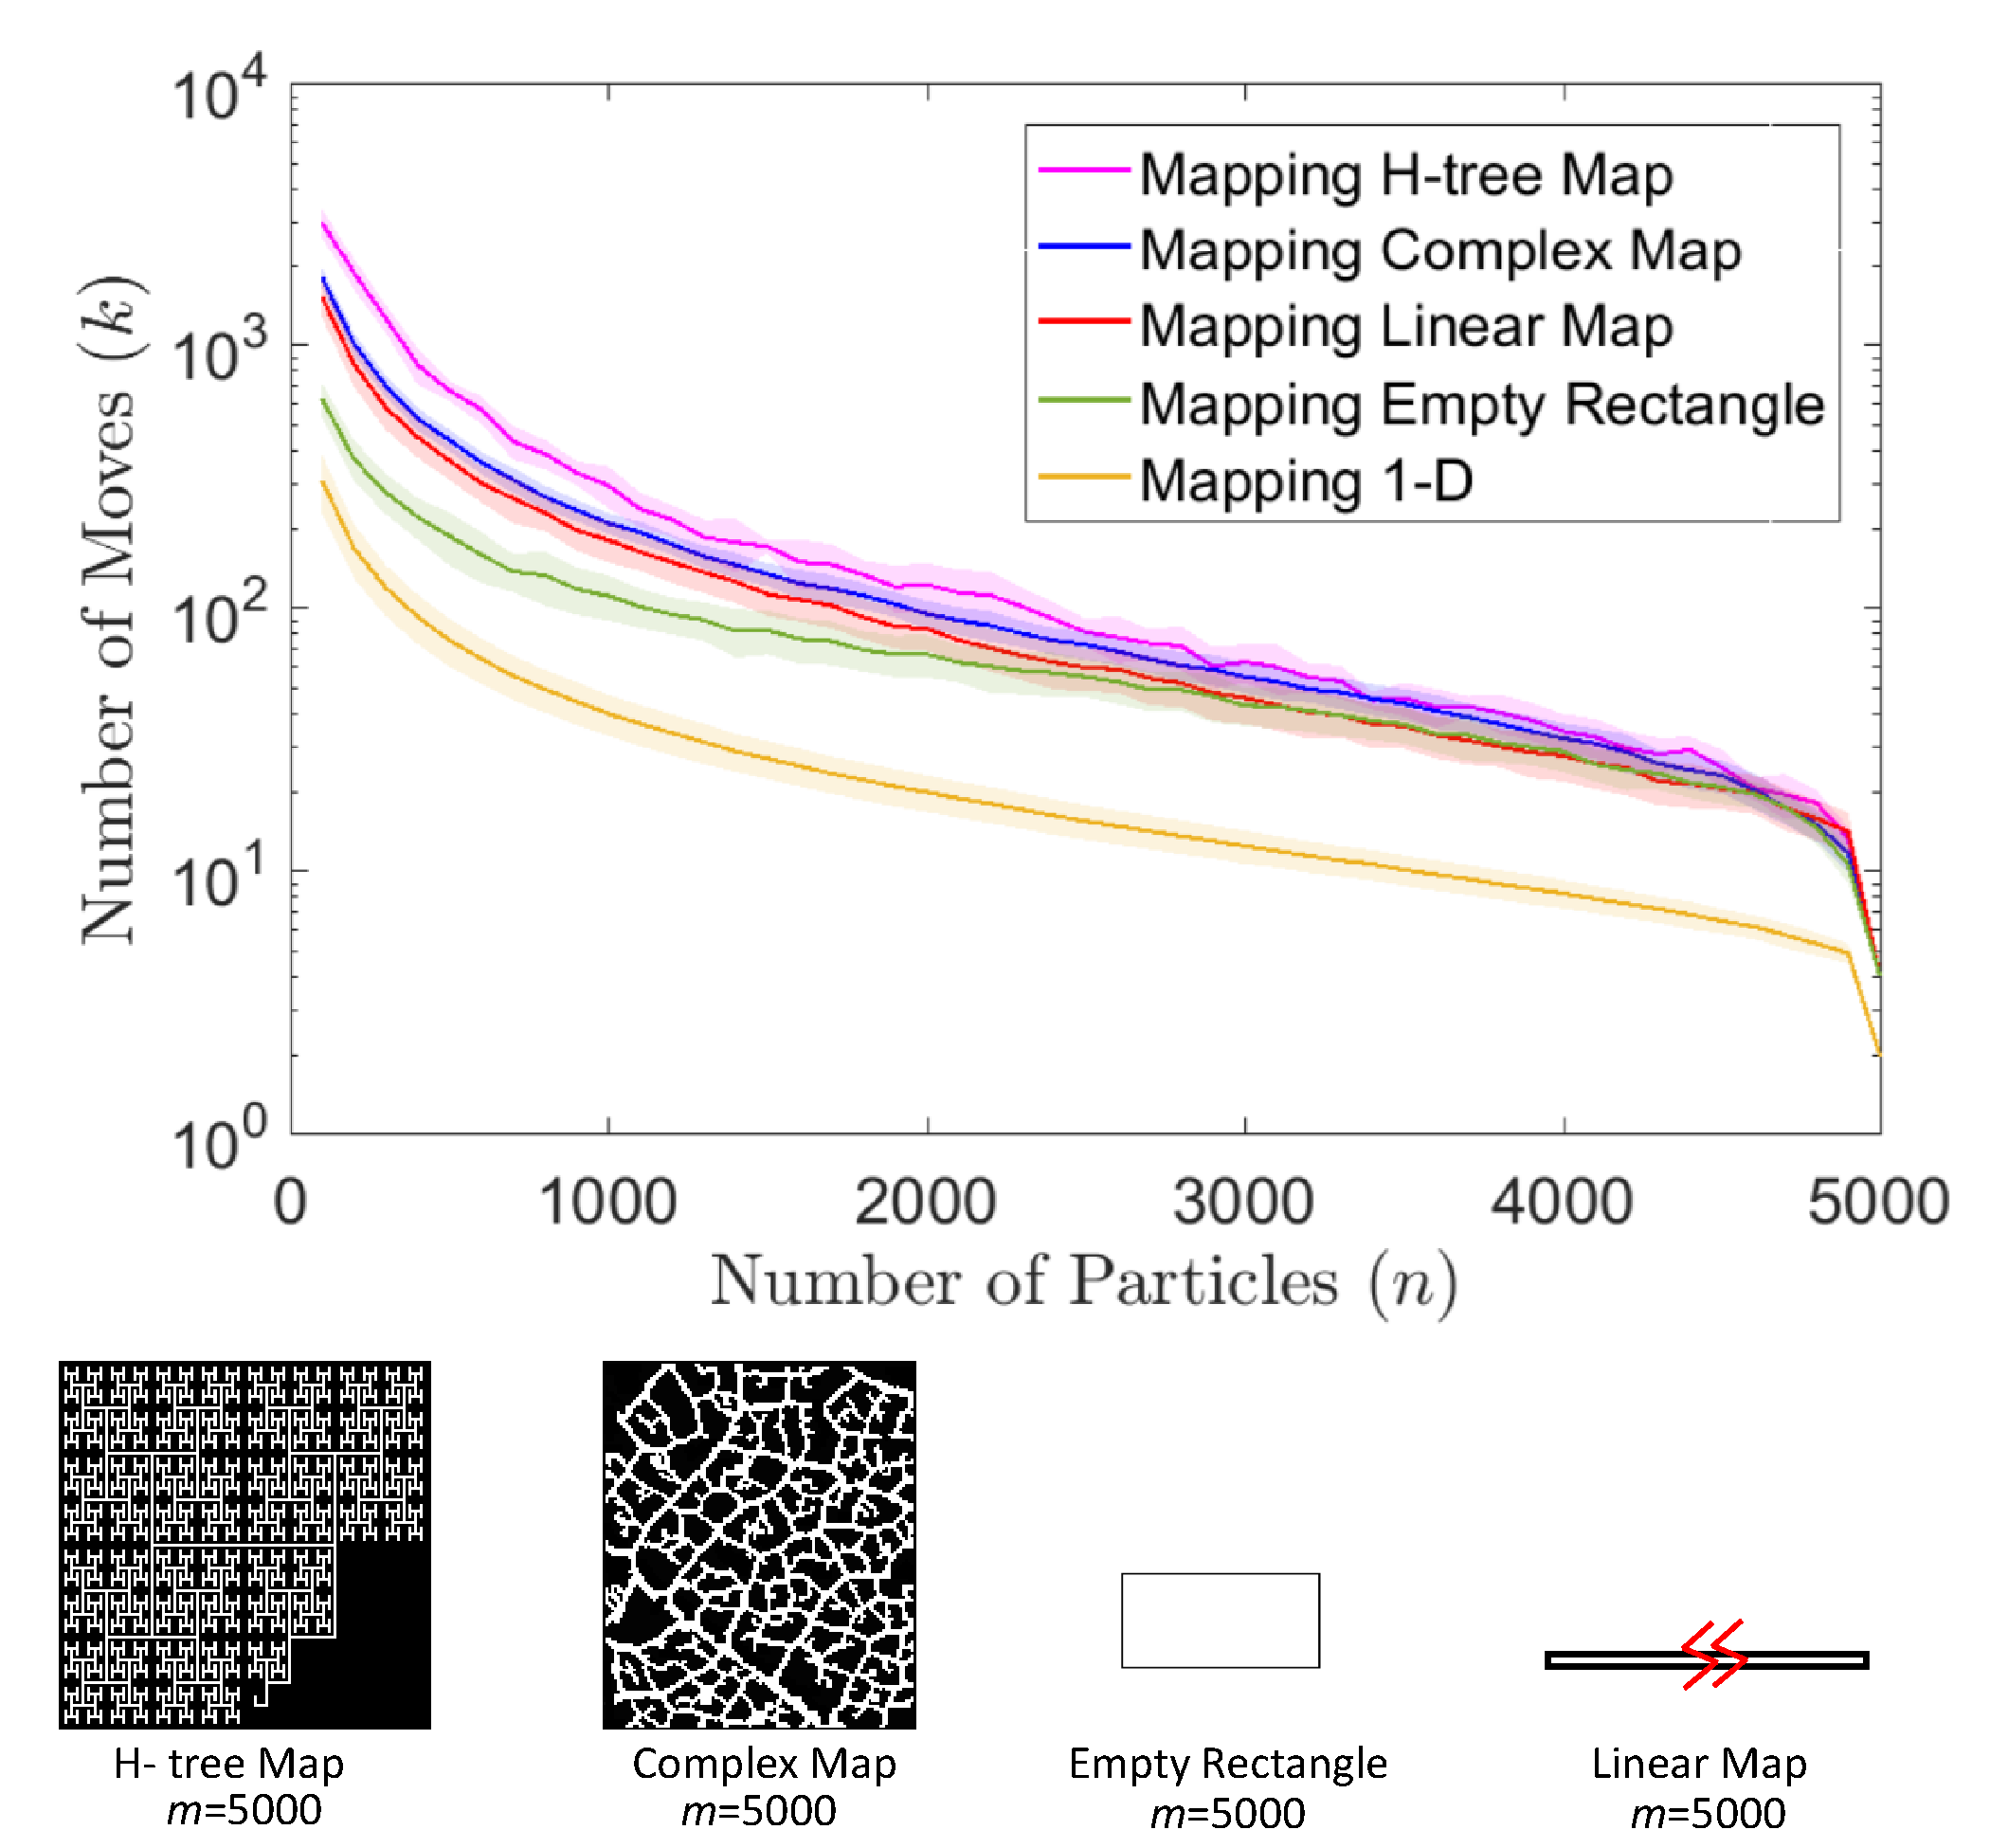
\includegraphics[width=1.0\columnwidth]{MappingAlg3maps}
\end{center}
\caption{\label{fig:MappingAlg3maps}
Comparison of mapping using the {\sc ClosestFrontier} algorithm on 2D maps of four types and 1D mapping on a linear map. 
Each map has 5000 free cells.
}
\end{figure}

 %%%%%%%%%%%%%%%  FrontierNodesVsk.pdf
The difference between algorithms is highlighted in Fig.~\ref{fig:FrontierNodesVsk}, which shows the number of frontier cells as a function of the number of moves commanded. All tests used $n=1000$ particles. {\sc ElectParticle} requires on average twice as many moves as {\sc ClosestFrontier} and {\sc RandomMoves} requires ten times as many moves as {\sc ClosestFrontier}.
The deviations for the {\sc ClosestFrontier} are also much less than the other two as seen from Fig.~\ref{fig:FrontierNodesVsk} and Fig.~\ref{fig:Alg_linlogplot}.
	
\begin{figure}
\begin{center}
	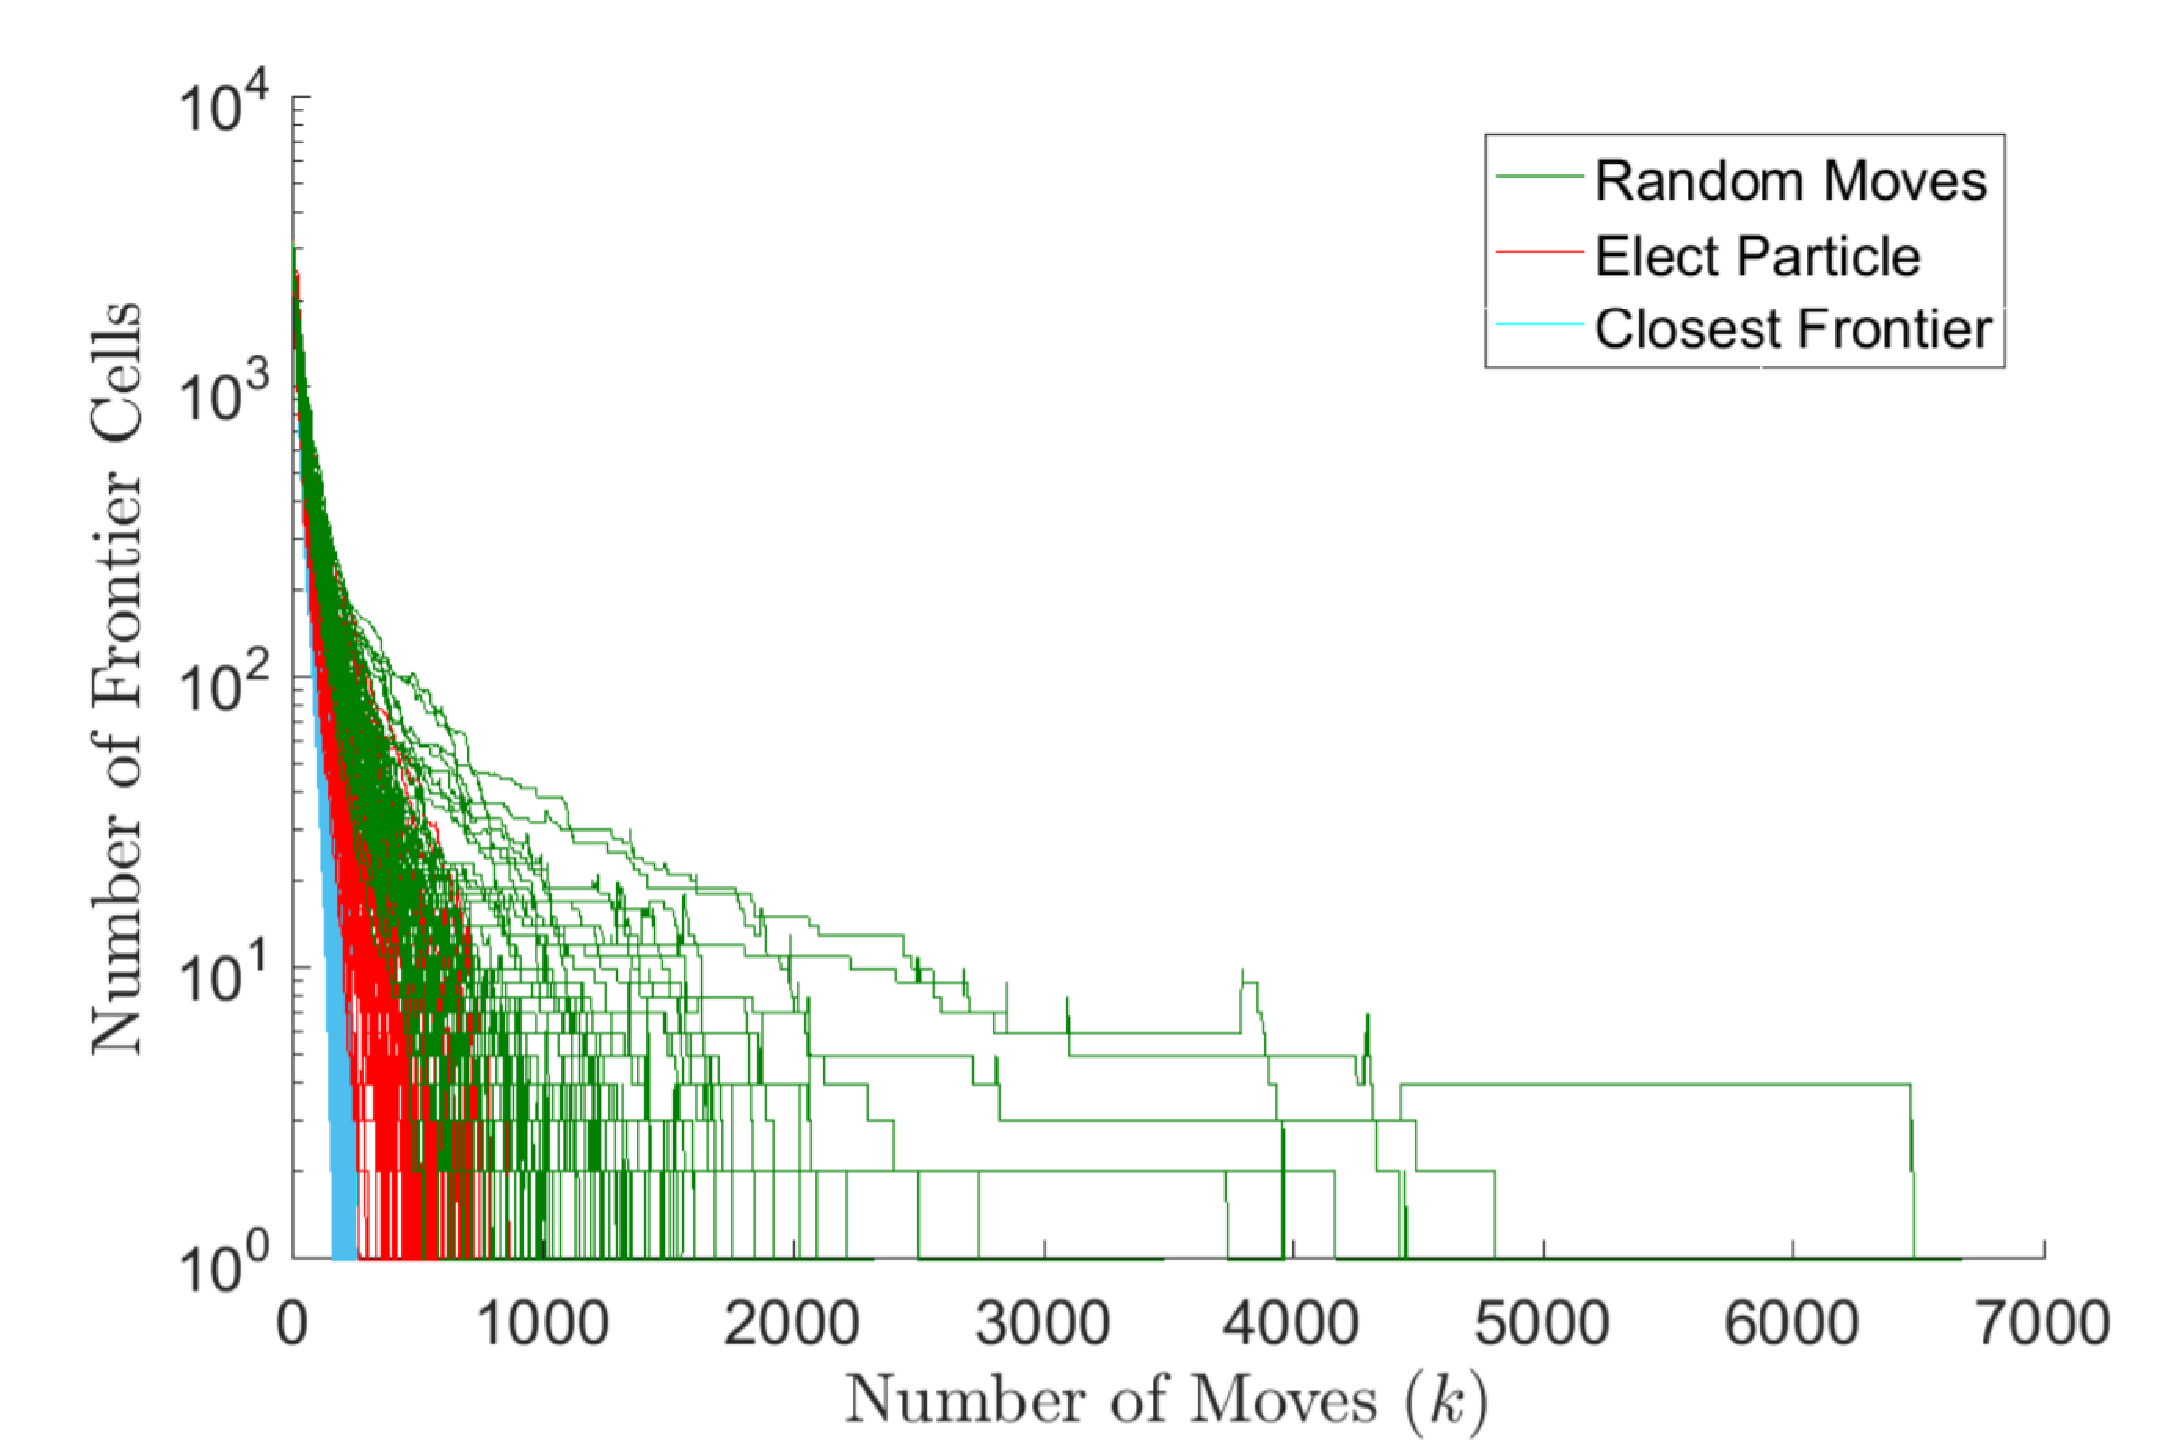
\includegraphics[width=1.0\columnwidth]{FrontierNodesVsklinlog.pdf}
\end{center}
\vspace{-2em}
\caption{\label{fig:FrontierNodesVsk}
Performing mapping on the complex 2D map with $n=1000$ particles. {\sc RandomMoves} requires 1683 moves, {\sc ElectParticle} requires 578 moves and {\sc ClosestFrontier} requires 215 moves on average}
\end{figure}	


%%%%%%%%%%%%%%%  fig:Alg_linlogplot

Fig.~\ref{fig:Alg_linlogplot} compares the performance of {\sc RandomMove}, {\sc ElectParticle}, and {\sc ClosestFrontier} on the complex 2D map. 
 For all algorithms the mean completion time and standard deviation of the completion time decreased with increasing numbers of particles. 
{\sc RandomMoves} performs worst, with the largest number of required moves and the largest standard deviation of required moves. {\sc RandomMoves} is slightly better than {\sc ElectParticle} for large numbers of particles, but both algorithms are beat by {\sc ClosestFrontier}, which has the minimum number of required moves and the smallest standard deviation.
  The maximum number of moves required using the {\sc ClosestFrontier} algorithm was for $k$=100 with an average of $\approx$1816 moves and standard deviation of 160 moves.
This reduces to four moves with 0 standard deviation when $n$= 5000 (the total number of free spaces).
%  The log plot shows that all three algorithms have an almost logarithmic relationship between $m$, the number of free spaces, and $k$, the number of particles.    % I don�t think we can claim this.  You'd have to fit a logrithmic fit to the data.  Try to do this with the linear-linear version of this data -- is it logarithmic?

\begin{figure}
\begin{center}
	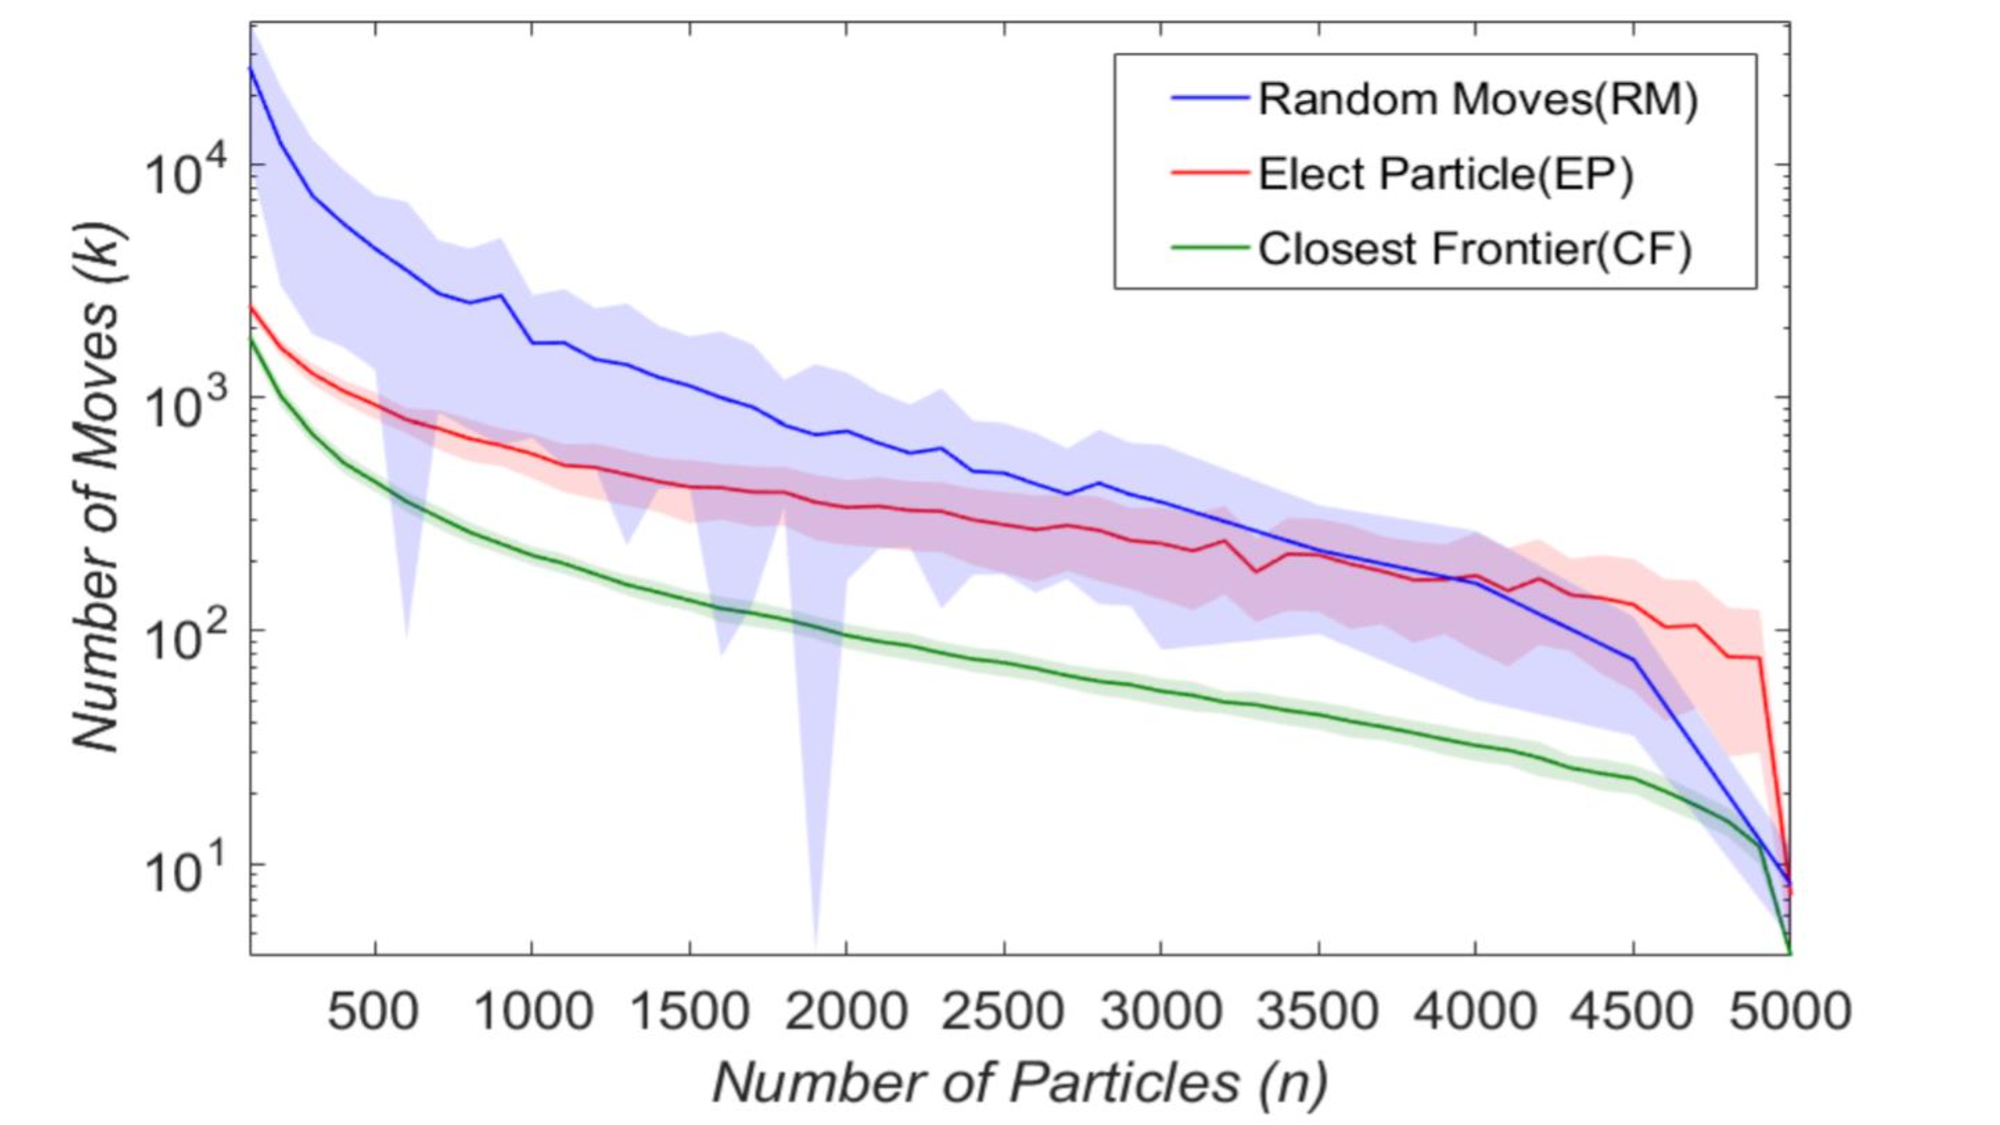
\includegraphics[width=1.0\columnwidth]{Alg_linlogplot}
\end{center}
\caption{\label{fig:Alg_linlogplot}
Comparison of three algorithms - {\sc RandomMoves}, {\sc ElectParticle} and {\sc ClosestFrontier} for mapping the 2D Complex Map of 5000 free spaces.}
\end{figure}

%%%%%%%%%%%%%%%  fig:CoverageMappingForaging
Fig.~\ref{fig:CoverageMappingForaging} compares mapping, coverage, and subset coverage on the complex 2D map. All trials used {\sc ClosestFrontier}. Coverage is performed with a known map, but with all free cells initialized to be frontier cells. Similarly, subset coverage has a known map, but 10\% of the empty cells are labeled as frontier cells. Subset coverage is easier than coverage and coverage is easier than mapping.

\begin{figure}
\begin{center}
\vspace{-8em}
	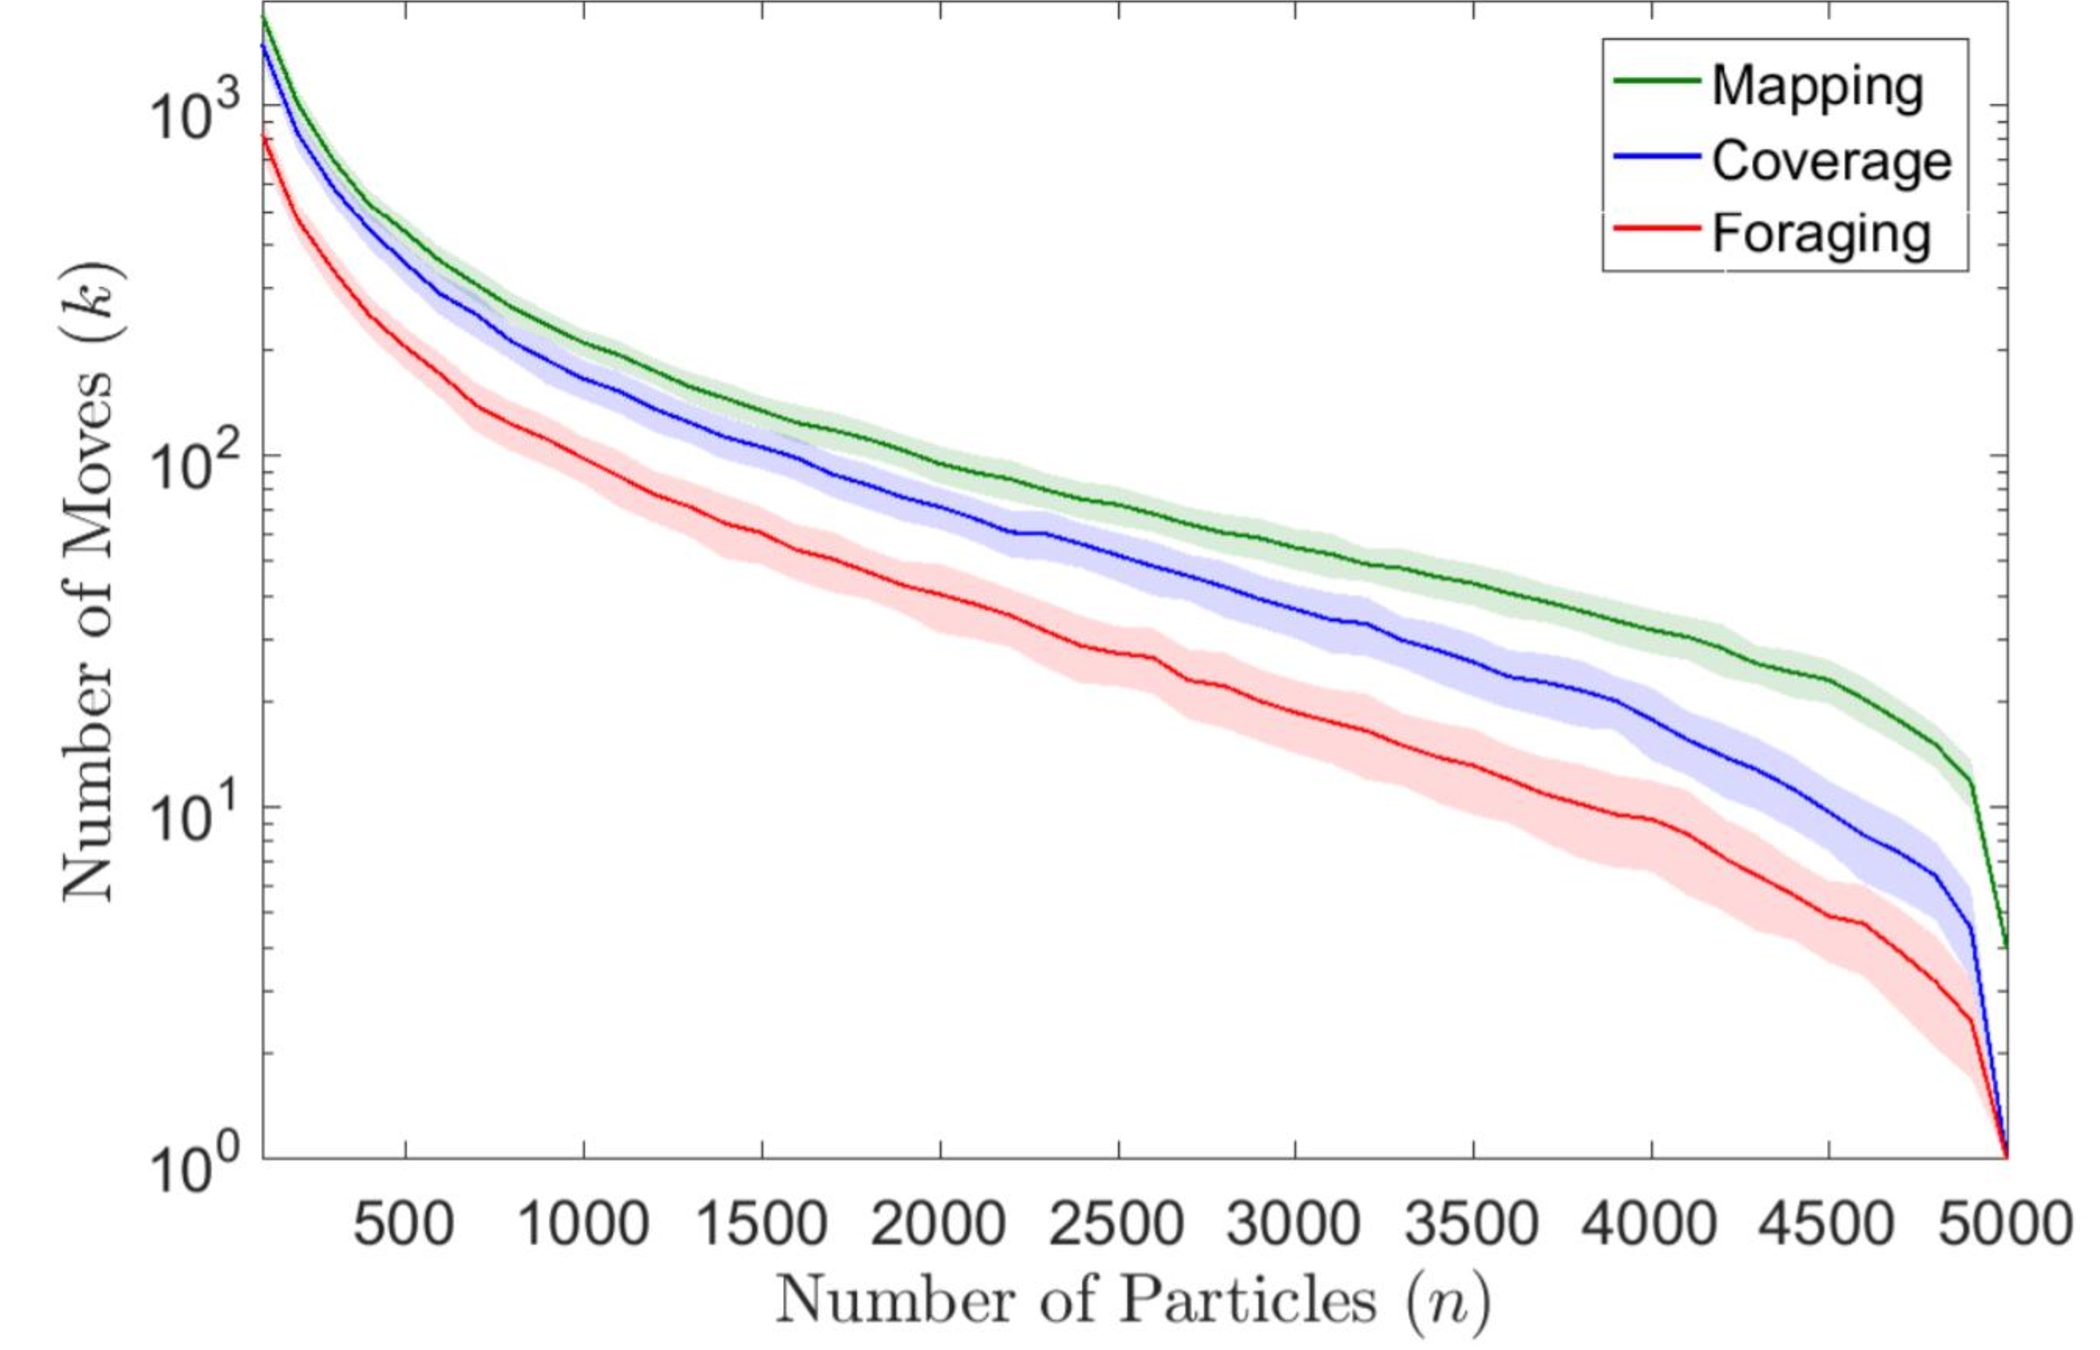
\includegraphics[width=1.0\columnwidth]{CoverageMappingForaging.pdf}
\end{center}
\vspace{-9em}
\caption{\label{fig:CoverageMappingForaging}
Comparison of three related problems: mapping, coverage, and subset coverage on the complex 2D map.}
\end{figure}


%%%%%%%%%%%%%%%  fig:RegionvsFloodvsUniform
The final simulation test, shown in Fig.~\ref{fig:RegionvsFloodvsUniform}, compares the effect of different initial particle distributions in the complex 2D map.  
$Region~fill$ places all $n$ particles at a minimum Manhattan distance from a randomly selected location on the map.
$Flood~fill$ places one particle at a randomly selected location in the free space, and places the remaining particles according to a breadth-first expansion inside the free space.
$Uniform~distribution$ places the particles uniformly randomly.  
$Region~fill$ and $flood~fill$ have similar performance, while $uniform~distribution$ requires many fewer moves. 
This is because dispersing particles using only uniform inputs is difficult, and a $uniform~distribution$ starts with the particles dispersed, which allows it to map much faster.
\begin{figure}
\begin{center}
	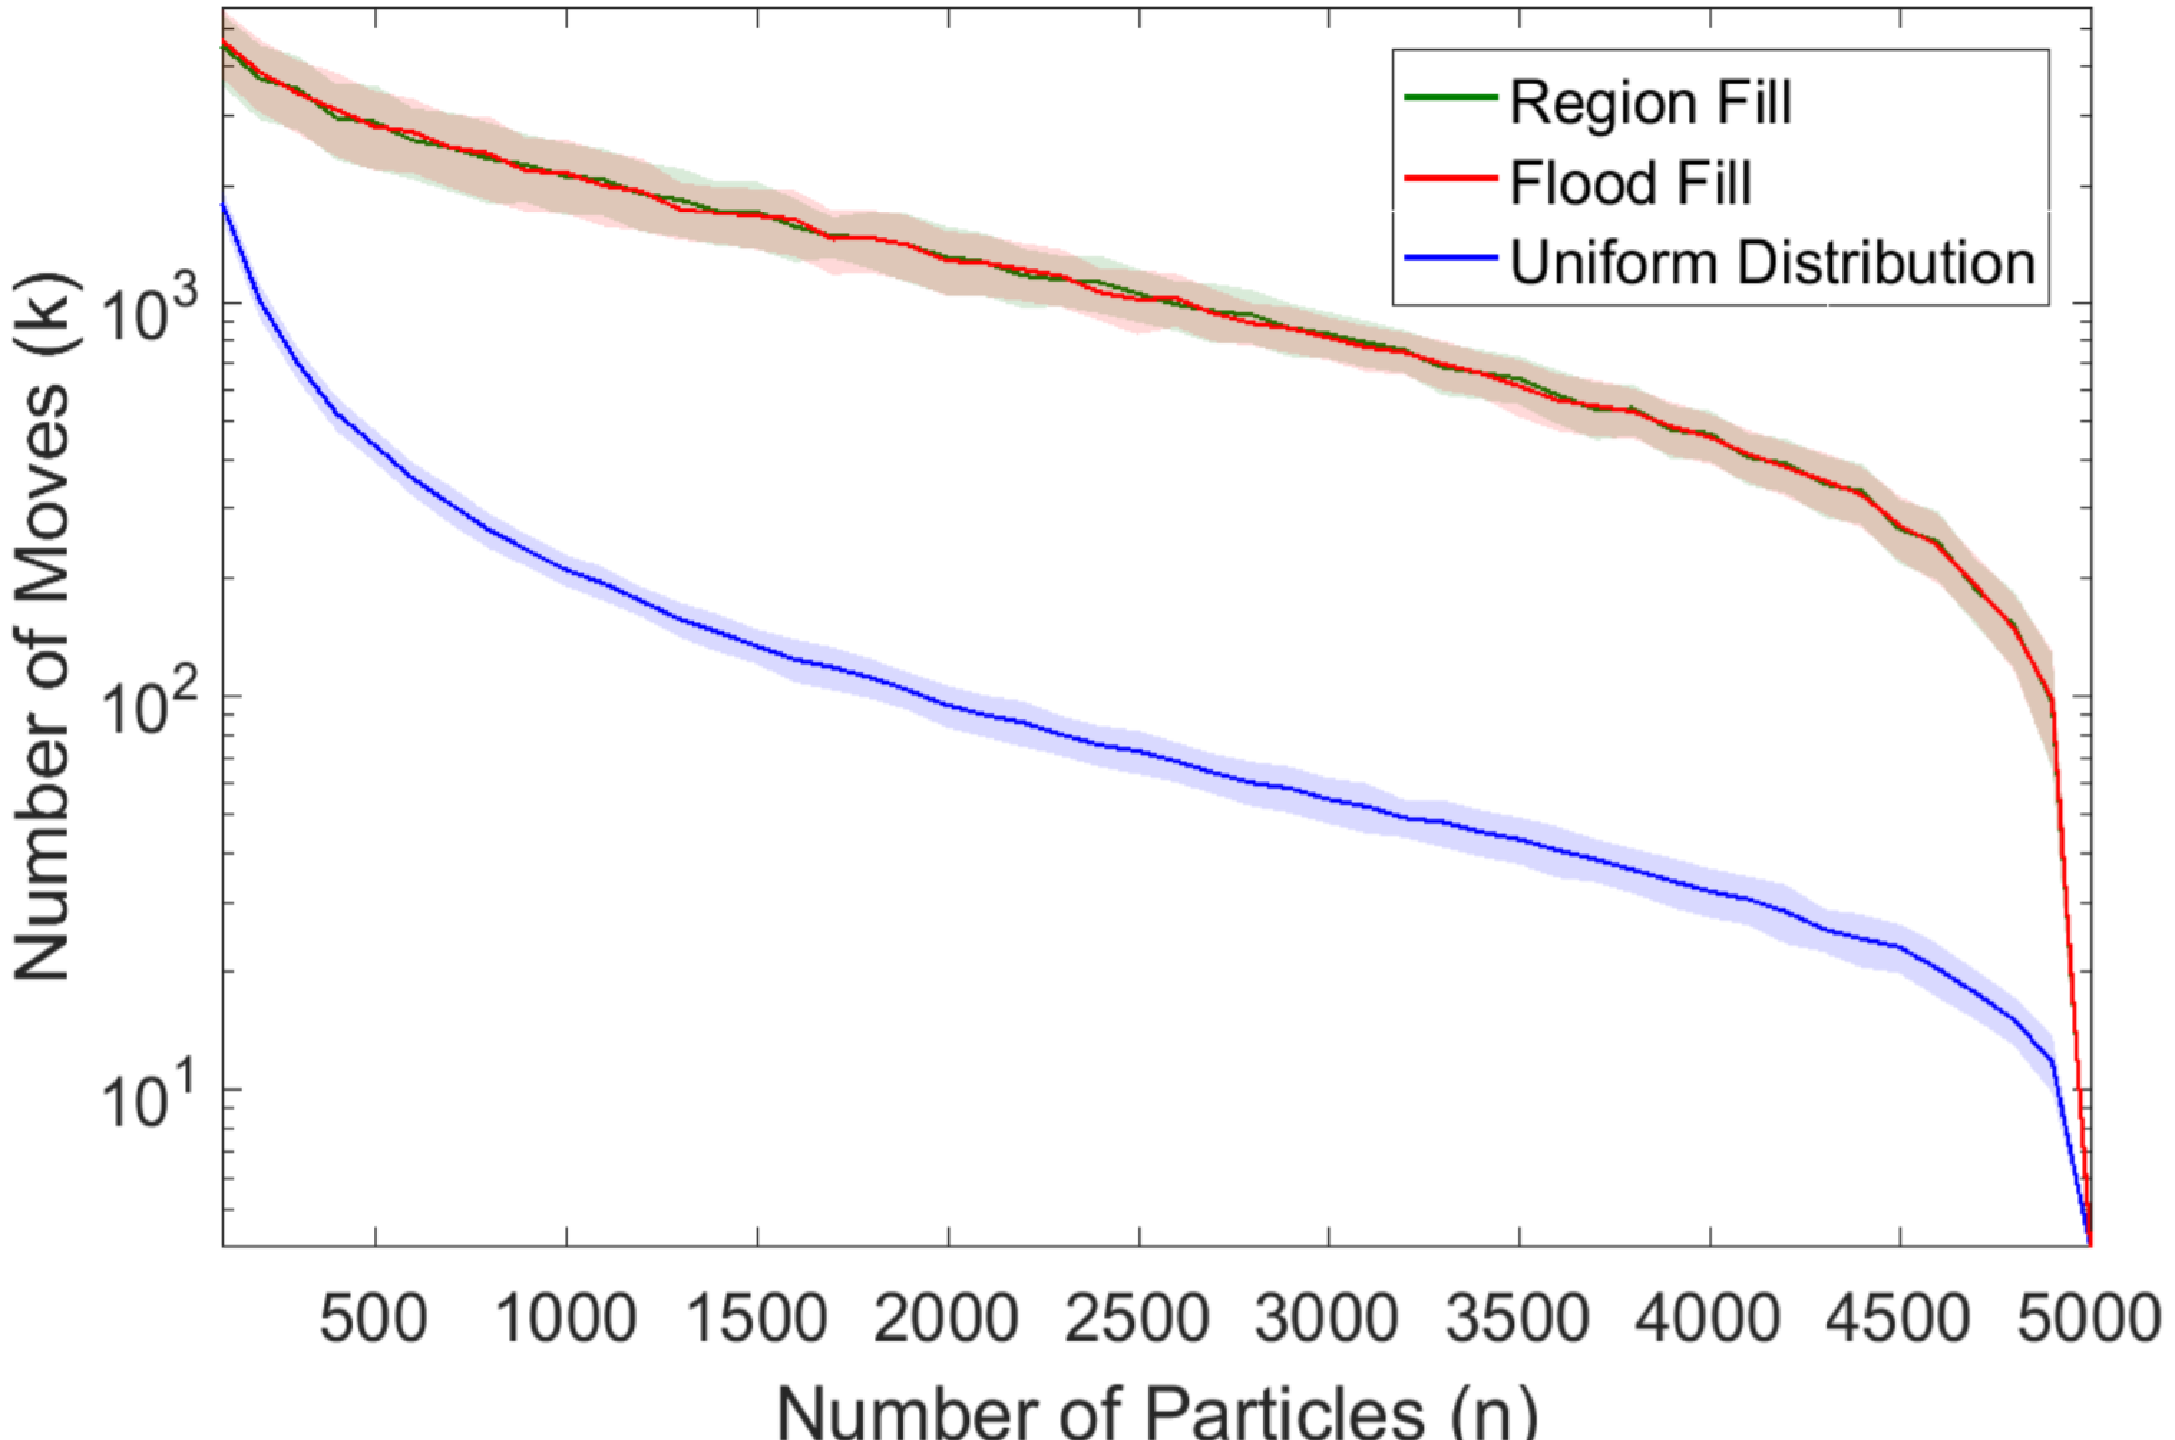
\includegraphics[width=1.0\columnwidth]{RegionvsFloodvsUniform.pdf}
\end{center}
\caption{\label{fig:RegionvsFloodvsUniform}
Comparison with different distributions: $flood~fill$, $region~fill$, and $uniform~distribution$ for mapping on the complex 2D map. The results for $flood~fill$ and $region~fill$ overlap. }
\end{figure}









%%%%%%%%%%%%%%%
%%%%%%%%%%%%%%%
%
%%%%%%%%%%%%%%%%%%%%%%%%%%%%%%%%%%%%%%%%%%%%%%%%%%%%%%%%%%%
\section{experiment}\label{sec:expResults}
%%%%%%%%%%%%%%%%%%%%%%%%%%%%%%%%%%%%%%%%%%%%%%%%%%%%%%%%%%%
   % sadly, no experiment
%%%%%%%%%%%%%%%
%%%%%%%%%%%%%%%%%%%%%%%%%%%%%%%%%%%%%%%%%%%%%%%%%%%%%%%%%%%
\section{Conclusion and Future Work}\label{sec:conclusion}
%%%%%%%%%%%%%%%%%%%%%%%%%%%%%%%%%%%%%%%%%%%%%%%%%%%%%%%%%%%

This paper presented techniques for controlling particle swarms in 1D and 2D grids.
These particles can be tracked and controlled by an external agent, but control inputs are applied uniformly so that each particle experiences the same applied forces. 

We provided theoretical and practical insights  with potential relevance for fast MRI scans with magnetically controlled contrast media.
In particular, we developed an approach for searching for an object at an unknown distance $D$, where the search is subject to two different and independent cost parameters
for {\em moving} and for {\em measuring}. 
We showed that regardless of the relative cost of these two operations,
there is a simple $O(\log D/\log\log D)$-competitive strategy. Extending the 1D bicriterion to an arbitrary freespace polyomino is not straightforward,
as a two-dimensional scenario has to deal with more intricate topological and geometric difficulties. This leaves the analytic treatment as a future challenge.
This paper also presented benchmark algorithms for 2D mapping and coverage problems.
These results form a baseline for future work, which should focus on improving performance. 
Extensions to 3D and continuous spaces are especially relevant to the motivating problem of MR-scanning in living tissue.
%%%%%%%%%%%%%%%
%\section*{Acknowledgments}
%We thank Haoran Zhao, Jarrett Lonsford, An Nguyen, and Lillian Lin for help in making structures for the experiments. 
%Withheld for double-blind review
%%%%%%%%%%%%%%%
%% Use plainnat to work nicely with natbib. 

%\bibliographystyle{plainnat}
%\bibliographystyle{SageH}
\balance
\bibliographystyle{IEEEtran}
\bibliography{IEEEabrv,bib/uniformMapping,bib/more}


% Uncomment to add appendix:
%\input{appendix}

\end{document}
